\documentclass[times, utf8, zavrsni, numeric]{fer}
\usepackage{booktabs}
\usepackage{color}
\usepackage{listings}
\usepackage{siunitx}
\usepackage{textcomp}
\usepackage{multirow}
\usepackage{float}
\usepackage{array}
\usepackage{makecell}
\usepackage{tabularx}
\usepackage{graphicx}

\lstset{
    tabsize=4,
    basicstyle=\footnotesize\ttfamily,
    numbers=left,
    numbersep=1em,
    xleftmargin=2em,
    frame=single,
    framexleftmargin=2em,
    aboveskip=1.5em,
    belowskip=1em,
    breaklines=true,
    breakatwhitespace=false,
    showstringspaces=false,
    captionpos=b,
    literate=%
    {ÿ}{{\"y}}1
    	{Ø}{{\"O}}1
    	{Ù}{{\"U}}1
}

\renewcommand{\lstlistingname}{Isječak koda}

\newcommand{\rot}[1]{\rotatebox{90}{#1}}
\newcommand{\rotbf}[1]{\rotatebox{90}{\textbf{#1}}}

\graphicspath{{slike/}}

\let\labelitemi\labelitemii

\begin{document}

% TODO: Navedite broj rada.
\thesisnumber{2021-72}

% TODO: Navedite naslov rada.
\title{Programska potpora za upravljanje kamerom na CubeSat nanosatelitu}

% TODO: Navedite vaše ime i prezime.
\author{Nikola Gudan}

\maketitle

% Ispis stranice s napomenom o umetanju izvornika rada. Uklonite naredbu \izvornik ako želite izbaciti tu stranicu.
\izvornik

% Dodavanje zahvale ili prazne stranice. Ako ne želite dodati zahvalu, naredbu ostavite radi prazne stranice.
\zahvala{Hvala Karli Salamun na savjetima i pomoći pri izradi ovog rada. \\ Hannon allen. Savo 'lass a lalaith.}

\tableofcontents

\chapter{Uvod}
Projekt FERSAT, koji se od 2018. godine provodi na Fakultetu elektrotehnike i računarstva, uključuje izradu, lansiranje i korištenje jednog nanosatelita CubeSat. Satelit u izradi dimenzija je približno 10 cm x 10 cm x 10 cm, volumena jedne litre i ne teži od 4/3 kilograma, što ga svrstava u skupinu satelita formata CubeSat 1U \cite{fersat_stranica_projekta}. Očekivani životni vijek satelita je 3 godine, a bit će postavljen u Zemljinoj orbiti na visini između 500 i 600 kilometara. Planirani korisni teret \engl{payload} FERSAT-a podijeljen je na tri podsustava:

    \begin{itemize}
        \item kamera za snimanje površine Zemlje i zemaljskog horizonta,
        \item detektori svjetla u vidljivom i ultraljubičastom dijelu spektra za mjerenje svjetlosnog onečišćenja i debljine stupca ozona,
        \item komunikacijski sustav u radijskom X-pojasu (10.45 GHz) za prijenos podataka na Zemlju.
    \end{itemize}

    Radom korisnog tereta upravlja \textit{Payload Data Handler} (PDH) računalo. Zadaća je PDH računala prikupiti podatke iz senzorskog podsustava i kamere, pohraniti ih u trajnu memoriju \engl{non-volatile memory} te poslati te podatke na Zemlju korištenjem komunikacijskog podsustava. Kao PDH računalo odabran je mikrokontroler STM32L471VGT6 proizvođača ST Microelectronics.

    Za rad ostalih podsustava satelita koji nisu direktno vezani uz koristan teret (npr. upravljanje položajem satelita, slanje telemetrijskih podataka na Zemlju) brine se \textit{Command and Data Handler} (CDH) računalo. CDH računalo također upravlja napajanjem korisnog tereta i šalje naredbe PDH računalu. Komunikacija CDH i PDH računala odvija se korištenjem sučelja CAN (\textit{Controller Area Network}). Konkretno CDH računalo u trenutku pisanja ovog teksta još nije odabrano.
\chapter{Arhitektura sustava}

Slanjem određenog signala na sklop za kameru može se uslikati slika, a nakon slikanja slika se spremi na vlastiti međuspremnik kamere. Cilj je spremljenu kameru pročitati iz međuspremnika kamere i spremiti ju na \textit{flash} memoriju koja se nalazi na pločici PDH-a, gdje može biti spremljena dok se ne zatraži slanje slike preko X-band predajnika na Zemlju.

\textit{Flash} memorija, osim što služi za pohranu slike, služi i za pohranu podataka s drugih senzora. Ona prima i šalje podatke ovisno o poslanoj naredbi putem SPI komunikacije s mikrokontrolerom.

Upravljačko sklopovlje PDH računala se sastoji od STM32F471VGT6 mikrokontrolera, spomenute vanjske \textit{flash} memorije, konektora za povezivanje s ostalim dijelovima sustava (uključujući i konektor za povezivanje s kamerom), sustava za napajanje, upravljačkog sklopovlja za CAN komunikaciju i sklopa za kontrolu izvođenja programa (engl. \textit{watchdog}) \cite{zavrsni_filip_juric}. Izgled tiskane pločice upravljačkog sklopovlja PDH računala prikazan je na slikama \ref{fig:PDH_PCB_1} i \ref{fig:PDH_PCB_2}. Konektor X1 služi za povezivanje sustava s kamerom.

\begin{figure}[H]
	\centering
	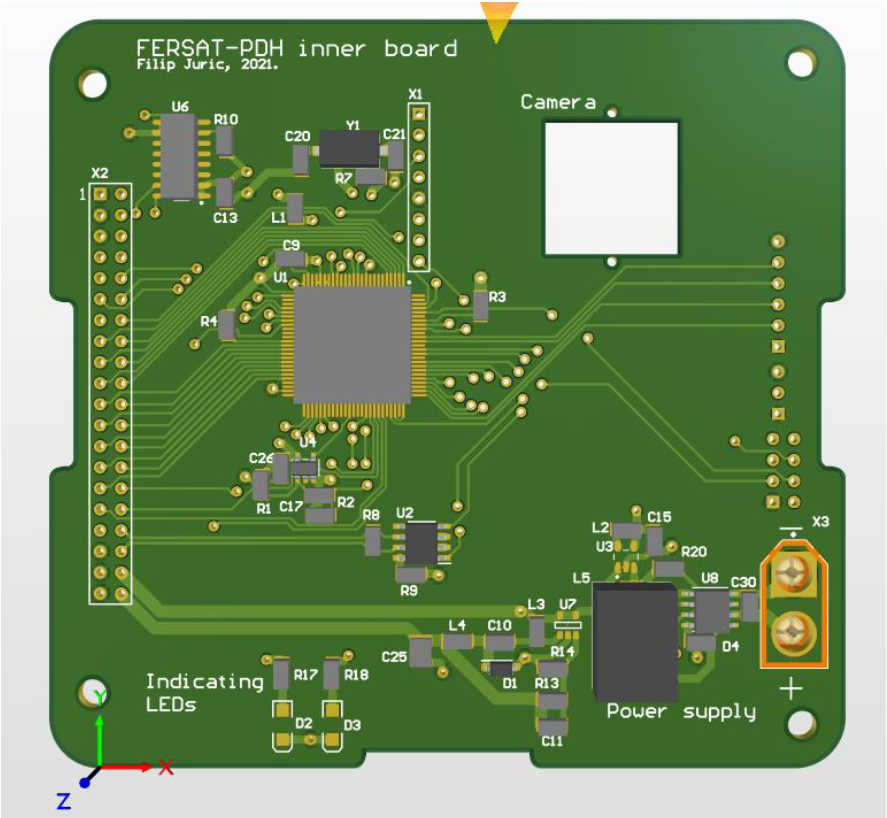
\includegraphics[height= 10 cm]{PDH_PCB_1.PNG}
	\caption{Prikaz gornje strane tiskane pločice upravljačkog sklopovlja PDH računala \cite{zavrsni_filip_juric}}
	\label{fig:PDH_PCB_1}
\end{figure}

\begin{figure}[H]
	\centering
	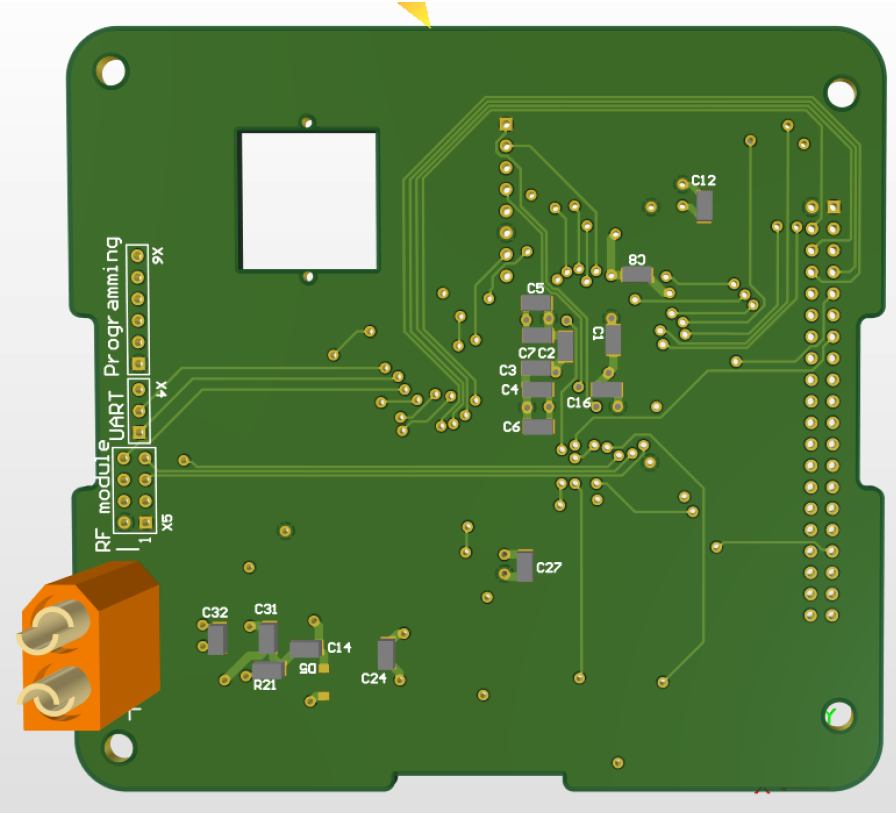
\includegraphics[height= 10 cm]{PDH_PCB_2.PNG}
	\caption{Prikaz donje strane tiskane pločice upravljačkog sklopovlja PDH računala \cite{zavrsni_filip_juric}}
	\label{fig:PDH_PCB_2}
\end{figure}

Programska podrška za PDH računalo već je razvijena \cite{diplomski_goran_petrak}. Međutim, u međuvremenu je došlo do promjene izbora mikrokontrolera PDH računala, te je stoga postojeću programsku podršku bilo potrebno prilagoditi trenutačnom sklopovlju.

S obzirom na prirodu ovog završnog projekta, gdje je naglasak bio na prilagođavanju postojeće programske podrške, u ovom radu će biti raspravljeni izazovi i izmjene do kojih je došlo tijekom prilagođavanja programske podrške. U poglavlju 2 dan je detaljan opis I\textsuperscript{2}C (engl. \textit{Inter-Integrated Circuit}) komunikacije, te su istaknute razlike između starog i novog sklopovlja koje su bile ključne za prilagođavanje programske podrške. Na isti način opisani su SPI (engl. \textit{Serial Peripheral Interface}) komunikacija i DMA (engl. \textit{Direct Memory Access}) prijenos u poglavlju x. Detaljan pregled razvijene programske podrške dan je u poglavlju y, gdje je opisana integracija programske podrške za kameru i \textit{flash} memorija u FreeRTOS operacijski sustav za rad u stvarnom vremenu.
\chapter{Sučelja za komunikaciju}

\section{I\textsuperscript{2}C sučelje}

Za konfiguraciju kamere Arducam 5MP Mini Plus, PDH računalo koristi I\textsuperscript{2}C komunikaciju. U nastavku slijedi općeniti opis I\textsuperscript{2}C protokola kao i razlike I\textsuperscript{2}C periferijskih sklopova između prethodno i trenutno korištenog mikrokontrolera (STM32F407VGT6, odnosno STM32L471VGT6).

\subsection{I\textsuperscript{2}C protokol}

I\textsuperscript{2}C je jednostavna dvosmjerna sinkrona serijska sabirnica razvijena od strane \textit{Philips Semiconductors} (sada \textit{NXP Semiconductors}) 1982. godine \cite{i2c_wikipedia}. Koristi dvije linije:
\begin{itemize}
	\item serijska podatkovna linija (SDA, \textit{Serial Data Line}),
	\item serijska linija signala takta (SCL, \textit{Serial Clock Line}).
\end{itemize}
Obje linije su pritegnute na visoku logičku razinu preko \textit{pull-up} otpornika. Moguće brzine prijenosa su:
\begin{itemize}
	\item do 100 kbit/s u \textit{Standard-mode} načinu rada, 
	\item do 400 kbit/s u \textit{Fast-mode} načinu rada,
	\item do 1 Mbit/s u \textit{Fast-mode Plus} načinu rada,
	\item do 3.4 Mbit/s u \textit{High-speed} načinu rada.
\end{itemize}
Navedene brzine se koriste kod dvosmjernog prijenosa, a moguća je i brzina do 5 Mbit/s u jednosmjernom prijenosu. Više uređaja se može spojiti na jednu sabirnicu, a svaki uređaj je prepoznatljiv po svojoj jedinstvenoj adresi i može se ponašati kao prijamnik ili odašiljač, ovisno o funkciji uređaja \cite{i2c_manual}. Protokol najčešće, a tako i u ovom slučaju, koristi 7-bitno adresiranje, a moguće je i korištenje 10-bitnog adresiranja. Osim konfiguracije prijamnika i odašiljača, uređaj također može biti \textit{master} uređaj ili \textit{slave} uređaj tijekom prijenosa podataka. \textit{Master} uređaj je uređaj koji inicijalizira prijenos podataka na sabirnici i generira signal takta kako bi omogućio prijenos. U tom trenutku, bilo koji uređaj koji je adresiran smatra se \textit{slave} uređajem.

Na I\textsuperscript{2}C sabirnicu se također može spojiti više \textit{master} uređaja, a primjer jednog takvog spoja sa dva mikrokontrolera dan je na slici \ref{fig:i2c_primjer_1}.
\begin{figure}[hp]
	\centering
	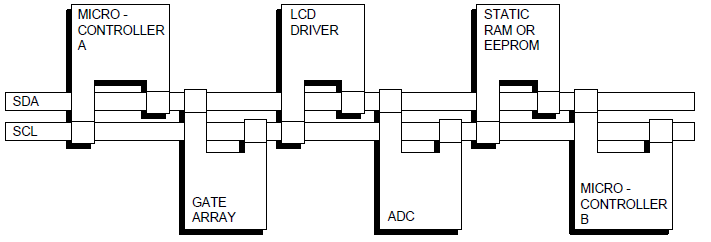
\includegraphics[width=\textwidth]{i2c_primjer_1.PNG}
	\caption{Primjer I\textsuperscript{2}C sabirnice sa spojena dva
	mikrokontrolera \cite{i2c_manual}}
	\label{fig:i2c_primjer_1}
\end{figure}
Prijenos podataka bi možda mogao izgledati ovako:
\begin{enumerate}
	\item Mikrokontroler A želi poslati podatke mikrokontroleru B:
	\begin{itemize}
		\item mikrokontroler A (\textit{master} uređaj) adresira mikrokontroler B (\textit{slave} uređaj)
		\item mikrokontroler A (\textit{master}-odašiljač) šalje podatke mikrokontroleru B (\textit{slave} uređaj-prijamnik)
		\item mikrokontroler A prekida prijenos
	\end{itemize}
	\item Mikrokontroler A želi primiti podatke sa mikrokontrolera B:
		\begin{itemize}
		\item mikrokontroler A (\textit{master} uređaj) adresira mikrokontroler B (\textit{slave})
		\item mikrokontroler A (\textit{master}-prijamnik) prima podtke sa mikrokontrolera B (\textit{slave}-odašiljač)
		\item mikroknotroler A prekida prijenos.
	\end{itemize}
\end{enumerate}
U svakom od navedenih slučajeva mikrokontroler A je generirao takt i prekidao prijenos. Kod prijenosa podataka na I\textsuperscript{2}C sabirnici, \textit{master} uređaj uvijek generira signal takta. U ovom radu korišten je samo jedan mikrokontroler, odnosno \textit{master} uređaj, pa će se u daljnjem tekstu podrazumijevati samo taj slučaj.

\subsubsection{Opis komunikacije i vremenski dijagram}
I\textsuperscript{2}C komunikacija započinje sa \textit{start} simbolom i završava sa \textit{stop} simbolom. Komunikacijom se može čitati ili pisati ovisno o R/W bitu u adresi. Struktura adresiranja kod 7-bitne adrese je prikazana u tablici \ref{Tab:i2c_seven_bit_adressing}.
\begin{center}
	\begin{table}[H]
		\centering
		\caption{Struktura adresiranja kod 7-bitne adrese \cite{i2c_wikipedia}}
		\begin{tabular}{ | c | c | c | c | c | c | c | c | c | }
			\hline
			& \multicolumn{7}{|c|}{Adresno polje} & R\textbackslash W \\
			\hline
			Pozicija bita u bajtu & 7 & 6 & 5 & 4 & 3 & 2 & 1 & 0 \\
			\hline
			Značenje & MSB & \multicolumn{5}{|c|}{} & LSB & 1=READ, 0=WRITE \\
			\hline
		\end{tabular}
		\label{Tab:i2c_seven_bit_adressing}
	\end{table}
\end{center}
Iz tablice je vidljivo da najmanje značajan bit označava želi li se podatak čitati ili pisati.

Imajući na umu izgled adresnog bajta, vremenski dijagram tipčne I\textsuperscript{2}C komunikacije prikazan je na slici \ref{fig:i2c_timing_diagram}.
\begin{figure}[hp]
	\centering
	
\includegraphics[width=\textwidth]{I2C_data_transfer.png}
	\caption{Vremenski dijagram I\textsuperscript{2}C komunikacije
	\cite{i2c_wikipedia}}
	\label{fig:i2c_timing_diagram}
\end{figure}
\begin{itemize}
	\item Prijenos podataka se inicijalizira \textit{start} uvjetom (S) tako da SDA linija prijeđe u nisku logičku razinu dok SCL linija ostaje u visokoj logičkoj razini.
	\item (Plavo područje) SCL prelazi u nisku logičku razinu i SDA postavlja prvi podatkovni bit dok je SCL u niskoj logičkoj razini.
	\item (Zeleno područje) Podaci se primaju dok SCL poraste za prvi bit (B\textsubscript{1}). Kako bi podaci bili valjani, SDA se ne smije promijeniti između rastućeg brida SCL-a i sljedećeg padajućeg brida.
	\item Postupak se ponavlja, SDA se postavlja dok je SCL u niskoj razini, a podaci se čitaju dok je SCL u visokoj razini (B\textsubscript{2} do B\textsubscript{n}).
	\item Nakon posljednjeg bita slijedi taktni impuls, tijekom kojeg SDA prelazi u nisku razinu pripremajući se za \textit{stop} uvjet.
	\item Signalizira se \textit{stop} uvjet kada SCL prijeđe u visoku logički razinu, nakon čega slijedi prelazak u visoku logičku razinu SDA signala.
	\item (Plavo područje) SCL prelazi u nisku logičku razinu i SDA postavlja
\end{itemize}
\textit{Start} i \textit{stop} uvjete uvijek generira \textit{master} uređaj. Nakon svakog bajta prijamnik šalje odašiljaču ACK bit kojim se signalizira uspješno primanje podatka, odnosno NACK bit kojim se signalizira neuspješno primanje podatka. ACK i NACK bitovi se nazivaju signalom potvrde i definiraju se na sljedeći način: odašiljač otpušta SDA liniju tijekom potvrdnog takta kako bi prijamnik mogao spustiti SDA na nisku razinu na kojoj i ostaje tijekom visoke razine takta. Ako SDA ostaje u visokoj razini tijekom devete periode takta, to predstavlja NACK (engl. \textit{Not Acknowledge}) signal, a suprotan slučaj predstavlja ACK (engl. \textit{Acknowledge}) signal. Ako je došlo do NACK signala, \textit{master} uređaj može generirati \textit{stop} uvjet kako bi prekinuo prijenos ili može ponovno generirati \textit{start} uvjet kako bi započeo novi prijenos. Vremenski dijagram cijele komunikacije s potvrdnim signalima prikazan je na slici \ref{fig:i2c_timing_diagram_transaction}.

\begin{figure}[hp]
	\centering
	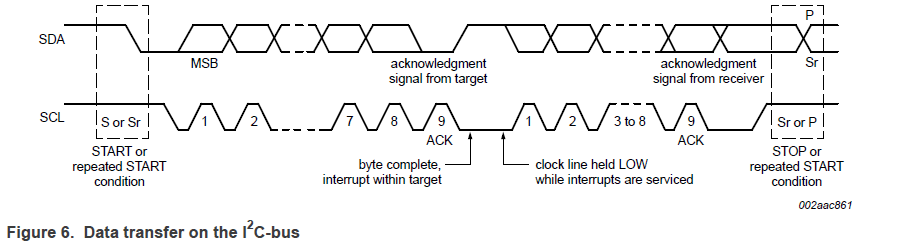
\includegraphics[width=\textwidth]{I2C_vremenski_dijagram.PNG}
	\caption{Prijenos podataka na I\textsuperscript{2}C sabirnici \cite{i2c_manual}}
	\label{fig:i2c_timing_diagram_transaction}
\end{figure}

\subsection{Razlika I\textsuperscript{2}C periferije na STM32L471VGT6 i \newline STM32F407VGT6 mikrokontrolerima}

Tijekom prijenosa koda sa starog mikrokontrolera na novi, primjećeno je da postoji razlika između struktura I\textsuperscript{2}C periferija. Točnije, postoji razlika između registarskih mapa na dvama periferijama, koje su vidljive usporedbom tablica \ref{Tab:l471_i2c_register_map} i \ref{Tab:f407_i2c_register_map} (\textit{napomena}: u tablicama nisu prikazani svi registri, jer se neki registri niti ne koriste, ili se koriste samo tijekom konfiguracije periferija. Za puni prikaz tablica treba provijeriti dokumentacije mikrokontrolera \cite{f407_manual}, \citep{l471_manual}).

\begin{table}[H]
	\caption{Registarska mapa I\textsuperscript{2}C periferije STM32L471VGT6 mikrokontrolera \cite{l471_manual}}
	\resizebox{\textwidth}{!}{%
	\begin{tabular}{|c|c|c|l|l|l|l|l|l|l|l|l|l|l|l|l|l|l|l|l|l|l|l|l|l|l|l|l|l|l|l|l|l|l|}
		\hline
		\textbf{Offset} & \textbf{\begin{tabular}[c]{@{}c@{}}Register\\ name\end{tabular}} & \rotbf{31} & \rotbf{30} & \rotbf{29} & \rotbf{28} & \rotbf{27} & \rotbf{26} & \rotbf{25} & \rotbf{24} & \rotbf{23} & \rotbf{22} & \rotbf{21} & \rotbf{20} & \rotbf{19} & \rotbf{18} & \rotbf{17} & \rotbf{16} & \rotbf{15} & \rotbf{14} & \rotbf{13} & \rotbf{12} & \rotbf{11} & \rotbf{10} & \rotbf{9} & \rotbf{8} & \rotbf{7} & \rotbf{6} & \rotbf{5} & \rotbf{4} & \rotbf{3} & \rotbf{2} & \rotbf{1} & \rotbf{0} \\
		\hline
		\multirow{2}{*}{0x0} & I2C\_CR1 & \multicolumn{8}{c|}{Res.} & \rot{PECEN} & \rot{ALERTEN} & \rot{SMBDEN} & \rot{SMBHEN} & \rot{GCEN} & \rot{WUPEN} & \rot{NOSTRETCH} & \rot{SBC} & \rot{RXDMAEN} & \rot{TXDMAEN} & \rot{Res.} & \rot{ANFOFF} & \multicolumn{4}{c|}{DNF[3:0]} & \rot{ERRIE} & \rot{TCIE} & \rot{STOPIE} & \rot{NACKIE} & \rot{ADDRIE} & \rot{RXIE} & \rot{TXIE} & \rot{PE} \\
		\cline{2-34}
		& Reset value & & & & & & & & & 0 & 0 & 0 & 0 & 0 & 0 & 0 & 0 & 0 & 0 & & 0 & 0 & 0 & 0 & 0 & 0 & 0 & 0 & 0 & 0 & 0 & 0 & 0 \\
		\hline
		\multirow{2}{*}{0x4} & I2C\_CR2 & \multicolumn{5}{c|}{Res.} & \rot{PECBYTE} & \rot{AUTOEND} & \rot{RELOAD} & \multicolumn{8}{c|}{NBYTES[7:0]} & \rot{NACK} & \rot{STOP} & \rot{START} & \rot{HEAD10R} & \rot{ADD10} & \rot{RD\_WRN} & \multicolumn{10}{c|}{SADD[9:0]} \\
		\cline{2-34}
		& Reset value & & & & & & 0 & 0 & 0 & 0 & 0 & 0 & 0 & 0 & 0 & 0 & 0 & 0 & 0 & 0 & 0 & 0 & 0 & 0 & 0 & 0 & 0 & 0 & 0 & 0 & 0 & 0 & 0 \\
		\hline
		\multirow{2}{*}{0x18} & I2C\_ISR & \multicolumn{8}{c|}{Res.} & \multicolumn{7}{c|}{ADDCODE[6:0]} & \rot{DIR} & \rot{BUSY} & \rot{Res.} & \rot{ALERT} & \rot{TIMEOUT} & \rot{PECERR} & \rot{OVR} & \rot{ARLO} & \rot{BERR} & \rot{TCR} & \rot{TC} & \rot{STOPF} & \rot{NACKF} & \rot{ADDR} & \rot{RXNE} & \rot{TXIS} & \rot{TXE} \\
		\cline{2-34}
		& Reset value & & & & & & & & & 0 & 0 & 0 & 0 & 0 & 0 & 0 & 0 & 0 & & 0 & 0 & 0 & 0 & 0 & 0 & 0 & 0 & 0 & 0 & 0 & 0 & 0 & 0 \\
		\hline
		\multirow{2}{*}{0x1C} & I2C\_ICR & \multicolumn{18}{c|}{Res.} & \rot{ALERTCF} & \rot{TIMOUTCF} & \rot{PECCF} & \rot{OVRCF} & \rot{ARLOCF} & \rot{BERRCF} & \multicolumn{2}{c|}{Res.} & \rot{STOPCF} & \rot{NACKCF	} & \rot{ADDRCF} & \multicolumn{3}{c|}{Res.} \\
		\cline{2-34}
		& Reset value & & & & & & & & & & & & & & & & & & & 0 & 0 & 0 & 0 & 0 & 0 & & & 0 & 0 & 0 & & & \\
		\hline
		\multirow{2}{*}{0x24} & I2C\_RXDR & \multicolumn{24}{c|}{Res.} & \multicolumn{8}{c|}{RXDATA[7:0]} \\
		\cline{2-34}
		& Reset value & & & & & & & & & & & & & & & & & & & & & & & & & 0 & 0 & 0 & 0 & 0 & 0 & 0 & 0 \\
		\hline
		\multirow{2}{*}{0x28} & I2C\_TXDR & \multicolumn{24}{c|}{Res.} & \multicolumn{8}{c|}{TXDATA[7:0]} \\
		\cline{2-34}
		& Reset value & & & & & & & & & & & & & & & & & & & & & & & & & 0 & 0 & 0 & 0 & 0 & 0 & 0 & 0 \\
		\hline
	\end{tabular}%
	}
	\label{Tab:l471_i2c_register_map}
\end{table}

\begin{table}[H]
	\caption{Registarska mapa I\textsuperscript{2}C periferije STM32F407VGT6 mikrokontrolera \cite{f407_manual}}
	\resizebox{\textwidth}{!}{%
	\begin{tabular}{|c|c|c|l|l|l|l|l|l|l|l|l|l|l|l|l|l|l|l|l|l|l|l|l|l|l|l|l|l|l|l|l|l|l|}
		\hline
		\textbf{Offset} & \textbf{\begin{tabular}[c]{@{}c@{}}Register\\ name\end{tabular}} & \rotbf{31} & \rotbf{30} & \rotbf{29} & \rotbf{28} & \rotbf{27} & \rotbf{26} & \rotbf{25} & \rotbf{24} & \rotbf{23} & \rotbf{22} & \rotbf{21} & \rotbf{20} & \rotbf{19} & \rotbf{18} & \rotbf{17} & \rotbf{16} & \rotbf{15} & \rotbf{14} & \rotbf{13} & \rotbf{12} & \rotbf{11} & \rotbf{10} & \rotbf{9} & \rotbf{8} & \rotbf{7} & \rotbf{6} & \rotbf{5} & \rotbf{4} & \rotbf{3} & \rotbf{2} & \rotbf{1} & \rotbf{0} \\
		\hline
		\multirow{2}{*}{0x0} & I2C\_CR1 & \multicolumn{16}{c|}{Res.} & \rot{SWRST} & \rot{Res.} & \rot{ALERT} & \rot{PEC} & \rot{POS} & \rot{ACK} & \rot{STOP} & \rot{START} & \rot{NOSTRETCH} & \rot{ENGC} & \rot{ENPEC} & \rot{ENARP} & \rot{SMBTYPE} & \rot{Res.} & \rot{SMBUS} & \rot{PE} \\
		\cline{2-34}
		& Reset value & & & & & & & & & & & & & & & & & 0 & & 0 & 0 & 0 & 0 & 0 & 0 & 0 & 0 & 0 & 0 & 0 & & 0 & 0 \\
		\hline
		\multirow{2}{*}{0x4} & I2C\_CR2 & \multicolumn{19}{c|}{Res.} & \rot{LAST} & \rot{DMAEN} & \rot{ITBUFEN} & \rot{ITEVTEN} & \rot{ITERREN} & \multicolumn{2}{c|}{Res.} & \multicolumn{6}{c|}{FREQ[5:0]} \\
		\cline{2-34}
		& Reset value & & & & & & & & & & & & & & & & & & & & 0 & 0 & 0 & 0 & 0 & & & 0 & 0 & 0 & 0 & 0 & 0 \\
		\hline
		\multirow{2}{*}{0x10} & I2C\_DR & \multicolumn{24}{c|}{Res.} & \multicolumn{8}{c|}{DR[7:0]} \\
		\cline{2-34}
		& Reset value & & & & & & & & & & & & & & & & & & & & & & & & & 0 & 0 & 0 & 0 & 0 & 0 & 0 & 0 \\
		\hline
		\multirow{2}{*}{0x14} & I2C\_SR1 & \multicolumn{16}{c|}{Res.} & \rot{SMBALERT} & \rot{TIMEOUT} & \rot{Res.} & \rot{PECERR} & \rot{OVR} & \rot{AF} & \rot{ARLO} & \rot{BERR} & \rot{TxE} & \rot{RxNE} & \rot{Res.} & \rot{STOPF} & \rot{ADD10} & \rot{BTF} & \rot{ADDR} & \rot{SB} \\
		\cline{2-34}
		& Reset value & & & & & & & & & & & & & & & & & 0 & 0 & & 0 & 0 & 0 & 0 & 0 & 0 & 0 & & 0 & 0 & 0 & 0 & 0 \\
		\hline
		\multirow{2}{*}{0x18} & I2C\_SR2 & \multicolumn{16}{c|}{Res.} & \multicolumn{8}{c|}{PEC[7:0]} & \rot{DUALF} & \rot{SMBHOST} & \rot{SMBDEFAUL} & \rot{GENCALL} & \rot{Res.} & \rot{TRA} & \rot{BUSY} & \rot{MSL} \\
		\cline{2-34}
		& Reset value & & & & & & & & & & & & & & & & & 0 & 0 & 0 & 0 & 0 & 0 & 0 & 0 & 0 & 0 & 0 & 0 & & 0 & 0 & 0 \\
		\hline
	\end{tabular}%
	}
	\label{Tab:f407_i2c_register_map}
\end{table}

Vidljiva je razlika između količine registara, raspodjele i značenja njihovih bitova, kao i njihovih imena, što implicira različite funkcionalnosti pojedinih registara. Tako, npr. I\textsuperscript{2}C periferija kod STM32F407VGT6 sadržava 2 status registra: I2C\_SR1 i I2C\_SR2, dok kod STM32L471VGT6 postoji samo jedan status registar I2C\_ISR. Ta razlika je bitna zato što se tijekom prijenosa podataka na I\textsuperscript{2}C sabirnici trebaju provjeravati razne zastavice koje se mijenjaju tijekom komunikacije, kao što je npr. zastavica za prazni odašiljački registar (STM32F407VGT6: registar I2C\_SR1 bit 7, STM32L471VGT6: bit 0), zastavica za puni prijamnički registar (STM32F407VGT6: registar I2C\_SR1, bit 6, STM32L471VGT6: bit 2), zastavica za završetak prijenosa (STM32F407VGT6: ne postoji, STM32L471VGT6: bit 6) itd.

Vidljivo je također da kod STM32L471VGT6 postoji zastavica ADDR, koja inače kod STM32F407VGT6 signalizira uspješan primitak adrese uređaja mete, a kod \newline STM32L471VGT6 ta zastavica se koristi isključivo u \textit{slave} načinu rada, tako da ta zastavica nije bitna za ovaj projekt. Kako onda mikrokontroler zna da je poslana adresa točna? Naime, STM32L471VGT6 ima poseban registar za pohranu adrese uređaja mete, pa kada mikrokontroler pošalje \textit{start} uvjet on automatski nakon završetka \textit{start} uvjeta pošalje i adresu uređaja mete, a uspješan primitak adrese signalizira zastavica I2C\_ISR\_TXIS kod slanja podataka, odnosno I2C\_ISR\_RXNE zastavica kod primitka podataka.

Vidljive su i razlike u raspodjeli zastavica u registrima, kao i razlike u funkcijama koje zastavice signaliziraju. Inače bi te razlike stvarale probleme kod konfiguracije I\textsuperscript{2}C periferije, no, kako je tu brigu riješio kod generator ugrađen u STM32CubeIDE razvojno okruženje, nije bila posvećena pažnja tim razlikama. Način implementacije spomenutih razlika u programsku podršku opisan je u poglavlju z.

\section{SPI sučelje}

Protokol SPI se koristi za prijenos podataka između \textit{flash} memorije i mikrokontrolera, odnosno međuspremnika kamere. Kako bi se oslobodili resursi na mikrokontroleru, za prijenos podataka između kamere i \textit{flash} memorije se, u kombinaciji sa SPI protokolom, koristi i DMA prijenos. U ovom poglavlju bit će opisan SPI protokol i DMA prijenos i bit će istaknute razlike i problemi kod prilagođavanja programske podrške za STM32L471VGT6 mikrokontroler.

\subsection{SPI protokol}

SPI je sinkrono serijsko komunikacijsko sučelje koje se koristi za komunikaciju na kratkim udaljenostima, pretežito u ugradbenim računalnim sustavima \cite{spi_wikipedia}. 

SPI uređaji komuniciraju u \textit{full-duplex} načinu rada koristeći \textit{master-slave} arhitekturu, obično sa jednim \textit{master} uređajem. Više \textit{slave} uređaja može biti spojeno na jedan upravljač tako da se aktivira određeni \textit{chip select} signal za pojedini uređaj.

\subsubsection{Opis sučelja}

SPI sabirnica se sastoji od četiri signala:
\begin{itemize}
	\item SCLK: Serijski takt (izvor je \textit{master} uređaj),
	\item MOSI: \textit{Master Output Slave Input} (izvor podataka iz \textit{master} uređaja),
	\item MISO: \textit{Master Input Slave Output} (izvor podataka iz \textit{slave} uređaja),
	\item CS/SS: \textit{Chip/Slave Select} (aktivan nisko, signal iz \textit{master} uređaja, označava da se prenose podaci).
\end{itemize}
MOSI na \textit{master} uređaju se spaja na MOSI na \textit{slave} uređaju, dok se MISO na \textit{master} uređaju se spaja na MISO na \textit{slave} uređaju. CS/SS se koristi za pokretanje komunikacije između \textit{slave} i \textit{master} uređaja. Za svaki \textit{slave} uređaj postoji zaseban CS/SS priključak na \textit{master} uređaju. Takav način spajanja se naziva neovisni \textit{slave} uređaj. Primjer spajanja tri \textit{slave} uređaja na jedan \textit{master} uređaj u konfiguraciji neovisnog \textit{slave} uređaja prikazan je na slici \ref{fig:spi_three_slaves}.
\begin{figure}[H]
	\centering
	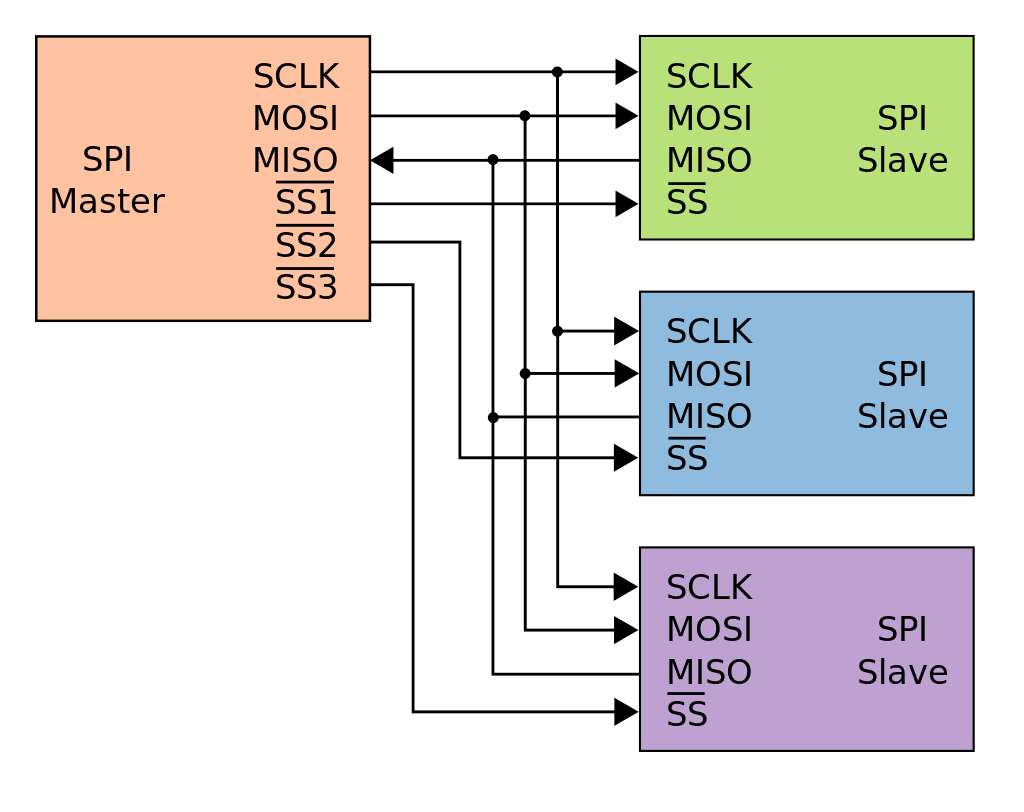
\includegraphics[height=7 cm]{SPI_three_slaves.svg.png}
	\caption{Spoj tri \textit{slave} uređaja na jedan \textit{master} uređaj u konfiguraciji neovisnog \textit{slave} uređaja. Vidljivo je da \textit{master} uređaj ima tri SS priključka, a svaki odgovara jednom \textit{slave} uređaju, dok se SCLK, MOSI i MISO linije međusobno dijele između \textit{slave} uređaja \cite{spi_wikipedia}}
	\label{fig:spi_three_slaves}
\end{figure}
Moguće je još spojiti uređaje u konfiguraciju ulančavanog \textit{slave} uređaja. U toj konfiguraciji \textit{slave} uređaji dijele isti CS/SS, a ulančavanjem preko MISO/MOSI linija podaci se prenose prema načelu posmačnog registra, koji je objašnjen u sljedećem potpoglavlju. Prikaz spajanja tri \textit{slave} uređaja se nalazi na slici \ref{fig:SPI_three_slaves_daisy_chained}.
\begin{figure}[H]
	\centering
	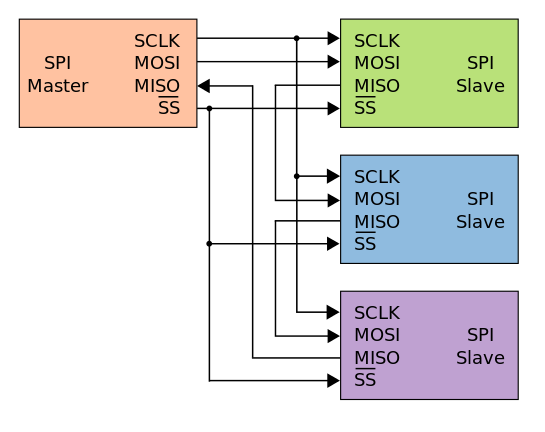
\includegraphics[height=7 cm]{SPI_three_slaves_daisy_chained.svg.png}
	\caption{Spoj tri \textit{slave} uređaja na jedan \textit{master} uređaj u konfiguraciji ulančavanog \textit{slave} uređaja \cite{spi_wikipedia}}
	\label{fig:SPI_three_slaves_daisy_chained}
\end{figure}

\subsubsection{Način rada}

SPI sabirnica radi s jednim \textit{master} uređajem i jednim ili više \textit{slave} uređaja. Ako se koristi jedan \textit{slave} uređaj, onda CS signal može biti postavljen u nisku logičku razinu, ako \textit{slave} uređaj to dopušta. Neki \textit{slave} uređaji zahtijevaju padajući brid CS signala kako bi započela komunikacija. Ako se koristi više \textit{slave} uređaja potreban je zaseban CS signal \textit{master} uređaja za svaki \textit{slave} uređaj.

\paragraph{Prijenos podataka}

Za početak komunikacije \textit{master} uređaj konfigurira takt koristeći frekvenciju koju podržava \textit{slave} uređaj, obično do nekoliko MHz. \textit{Master} uređaj zatim odabire \textit{slave} uređaj postavljanjem CS linije u nisko logičko stanje. Ako je potreban period čekanja, npr. za AD (analogno-digitalnu) pretvorbu, \textit{master} uređaj mora pričekati minimalno taj period vremena prije puštanja takta.

Tijekom svakog perioda takta obavlja se prijenos podataka u \textit{full-duplex} načinu rada. To znači da \textit{master} uređaj pošalje jedan bit na MOSI liniju, koji \textit{slave} uređaj pročita, dok u isto vrijeme \textit{slave} uređaj šalje jedan bit na MISO liniju, koji \textit{master} uređaj pročita. Takva sekvenca se održava čak i kada se izvodi jednosmjerni prijenos podataka.

Prijenosi podataka uključuju dva posmačna registra zadane veličine, npr. 8 bitova, jedan u \textit{master} i drugi u \textit{slave} uređaju. Registri su spojeni u topologiji virtualnog prstena (slika \ref{fig:spi_circular_transfer}).
\begin{figure}[H]
	\centering
	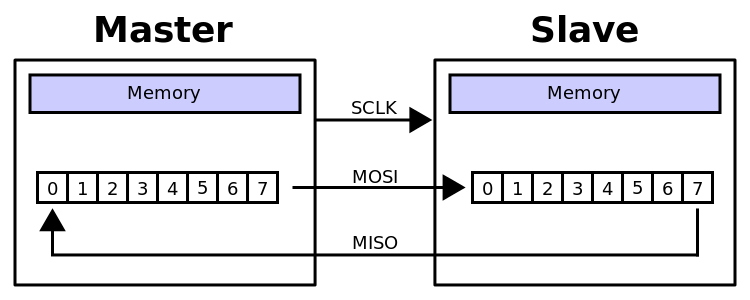
\includegraphics[width=\textwidth]{SPI_8-bit_circular_transfer.svg.png}
	\caption{Tipičan spoj dvaju posmačna registra koji formiraju kružni međuspremnik \cite{spi_wikipedia}}
	\label{fig:spi_circular_transfer}
\end{figure}
Podaci se obično pomiču tako da se prvo pomakne najznačajniji bit. Na brid takta, \textit{master} i \textit{slave} uređaj pomaknu bit i pošalju ga na prijenosnu liniju. Na sljedeći brid takta, na svakom prijamniku bit se uzorkuje s prijenosne linije i postavlja se kao novi najmanje značajni bit u posmačnom registru. \textit{Master} i \textit{slave} uređaji u potpunosti razmjene podatke u registrima nakon što se svi bitovi u registrima prebace. Ako je potrebno razmijeniti još podataka, posmačni registri se ponovno napune te se postupak ponavlja, a prijenos se može obavljati za bilo koji broj perioda takta. Kada je prijenos dovršen, \textit{master} uređaj prestaje davati takt i obično isključi CS signal, odnosno postavi ga na visoku razinu.

Prijenos se obično obavlja u riječima širine 8 bitova, no moguća je i širina riječi od 16 bita, ili čak 12 bitova, koji se koristi za digitalno-analogne i analogno-digitalne pretvornike.

\paragraph{Polaritet takta i faza}

Osim što mora podesiti frekvenciju takta, \textit{master} uređaj mora isto tako podesiti polaritet takta (CPOL, engl. \textit{Clock Polarity}) i fazu (CPHA, engl. \textit{Clock Phase}) ovisno o podacima. Vremenski dijagram je prikazan na slici \ref{fig:spi_timing_diagram}.
\begin{figure}[H]
	\centering
	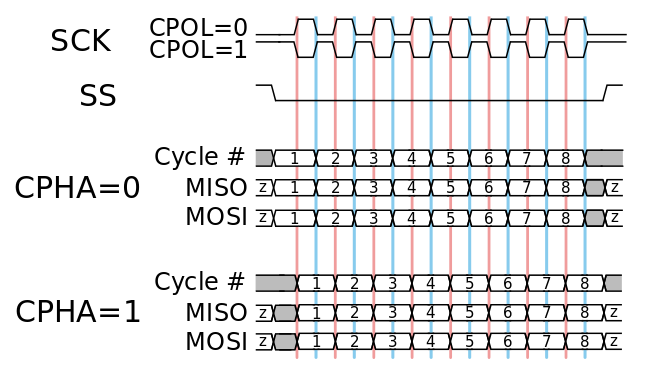
\includegraphics[height=7 cm]{SPI_timing_diagram2.svg.png}
	\caption{Vremenski dijagram koji pokazuje polaritet takta i fazu. Crvene linije označuju vodeće bridove, a plave linije označavaju prateće bridove \cite{spi_wikipedia}.}
	\label{fig:spi_timing_diagram}
\end{figure}
CPOL određuje polaritet kanala. Polaritet može biti invertiran jednostavnim inverterom.
\begin{itemize}
	\item Ako je CPOL = 0, onda takt miruje u niskom logičkom stanju, a svaki period se sastoji od impulsa visokog logičkog stanja. To znači da je vodeći brid rastući brid, a prateći brid padajući brid.
	\item Ako je CPOL = 1, onda takt miruje u visokom logičkom stanju, a svaki period se sastoji od impulsa niskog logičkog stanja. To znači da je vodeći brid padajući brid, a prateći brid rastući brid.
\end{itemize}
CPHA određuje fazu podatkovnih bitova u odnosu na takt.
\begin{itemize}
	\item Ako je CPHA = 0, strana koja šalje podatke mijenja podatak na prateći brid prethodnog perioda takta, dok strana koja prima podetke prihvaća podatak na (ili ubrzo nakon) vodeći brid perioda takta. Izlazna strana zadržava valjani podatak sve do pojave pratećeg brida trenutnog perioda takta.
	\item Ako je CPHA = 1, strana koja šalje podatke mijenja podatak na vodeći brid trenutnog perioda takta, dok strana koja prima podatke prihvaća podatak na (ili ubrzo nakon) pratećeg brida perioda takta. Izlazna strana zadržava valjani podatak do pojave vodećeg brida sljedećeg perioda takta. Na zadnji period, \textit{slave} uređaj zadržava valjani podatak na MISO liniji sve dok \textit{slave} uređaj ne bude deselektiran.
\end{itemize}
MOSI i MISO signali su obično stabilni za vrijeme pola perioda takta, sve do sljedeće promjene takta. SPI \textit{master} i \textit{slave} uređaji mogu uzorkovati podatke u bilo kojem vremenu unutar te polovice periode takta.

Kombinacije različitih konfiguracija CPOL i CPHA bitova predstavljaju načine rada. Konvecija je da CPOL predstavlja viši bit, dok CPHA predstavlja niži bit. Načini rada kod ARM-ovih mikrokontrolera su prikazani u tablici \ref{Tab:spi_modes}.
\begin{center}
	\begin{table}[H]
		\centering
		\caption{SPI načini rada kod ARM-ovih mikrokontrolera \cite{spi_wikipedia}}
		\begin{tabular}{| c | c | c |}
			\hline
			SPI način rada & CPOL & CPHA \\
			\hline
			0 & 0 & 0 \\
			\hline
			1 & 0 & 1 \\
			\hline
			2 & 1 & 0 \\
			\hline
			3 & 1 & 1 \\
			\hline
		\end{tabular}
		\label{Tab:spi_modes}
	\end{table}
\end{center}

\subsection{Prilagodba programske podrške sa STM32F407VGT6 mirokontrolera na STM32L471VGT6 mikrokontroler}

Što se tiče programske podrške za SPI komunikaciju između mikrokontrolera, \textit{flash} memorije i kamere, nije došlo do nikakvih poteškoća kod prijenosa programske podrške s prethodno korištenog mikrokontrolera na trenutni. Pogledom na blok dijagrame SPI periferije (slike \ref{fig:f407_spi_block_diagram} i \ref{fig:l471_spi_block_diagram}) vidljiva je velika sličnost između mikrokontrolera. Razlike između kontrolnih registara nisu problem, s obzirom na to da njih podešava generator koda, dok se razlike u statusnim registrima mogu zanemariti radi korištenja definicija registara i zastavica u programskoj podršci koju je pružao proizvođač mikrokontrolera.

Došlo je, međutim, do poteškoća kod prijenosa programske podrške za DMA prijenos, koje će biti objašnjene u sljedećem poglavlju.

\begin{figure}[H]
	\centering
	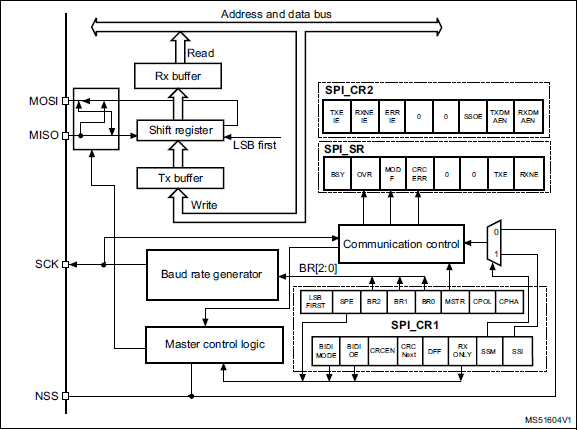
\includegraphics[width=\textwidth]{f407_spi_block_diagram.png}
	\caption{SPI blok dijagram mikrokontrolera STM32407VGT6 \cite[str. 876]{f407_manual}}
	\label{fig:f407_spi_block_diagram}
\end{figure}

\begin{figure}[H]
	\centering
	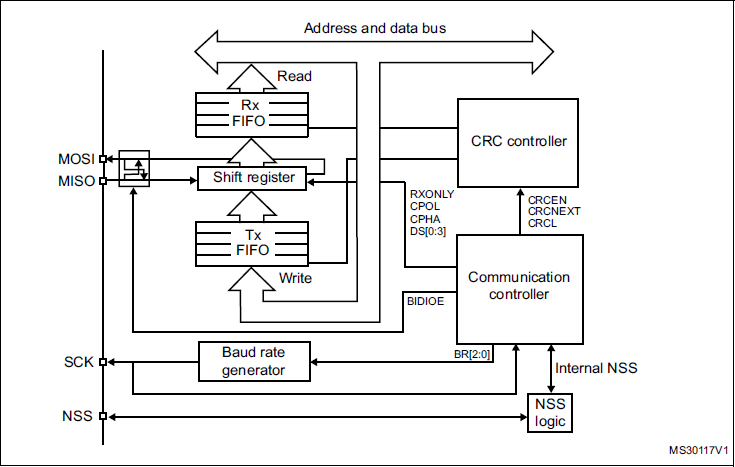
\includegraphics[width=\textwidth]{l471_spi_block_diagram.png}
	\caption{SPI blok dijagram mikrokontrolera STM32L471VGT6 \cite[str. 1451]{l471_manual}}
	\label{fig:l471_spi_block_diagram}
\end{figure}

%Razlike između SPI periferijskih sklopova STM32F407VGT6 i STM32L471VGT6 mikrokontrolera postoje, međutim, s obzirom na način koji se SPI protokol koristi u ovom projektu, te razlike su zanemarive i može se reći da SPI komunikacija na trenuračno korištenom mikrokontroleru funkcionira na isti način kao i na prethodno korištenom mikrokontroleru.

\subsection{DMA prijenos}

DMA se koristi kako bi se omogućio prijenos podataka visokih brzina između periferijskih sklopova i memorije ili između dviju memorijskih jedinica \cite{f407_manual}. Podatci se brzo mogu prenijeti bez posredovanja procesora. Na taj se način oslobađaju resursi procesora kako bi se mogle izvoditi druge operacije za vrijeme prijenosa.

U ovom projektu DMA prijenos se koristi između međuspremnika kamere i radne memorije mikrokontrolera.

\subsubsection{Razlike DMA periferije na STM32F407VGT6 i \\ STM32L471VGT6 mikrokontrolerima}

STM32F407VGT6 mikrokontroler ima dva DMA kontrolera. Blok dijagram jednog DMA kontrolera je prikazan na slici \ref{fig:f407_dma_block_diagram}.

\begin{figure}[H]
	\centering
	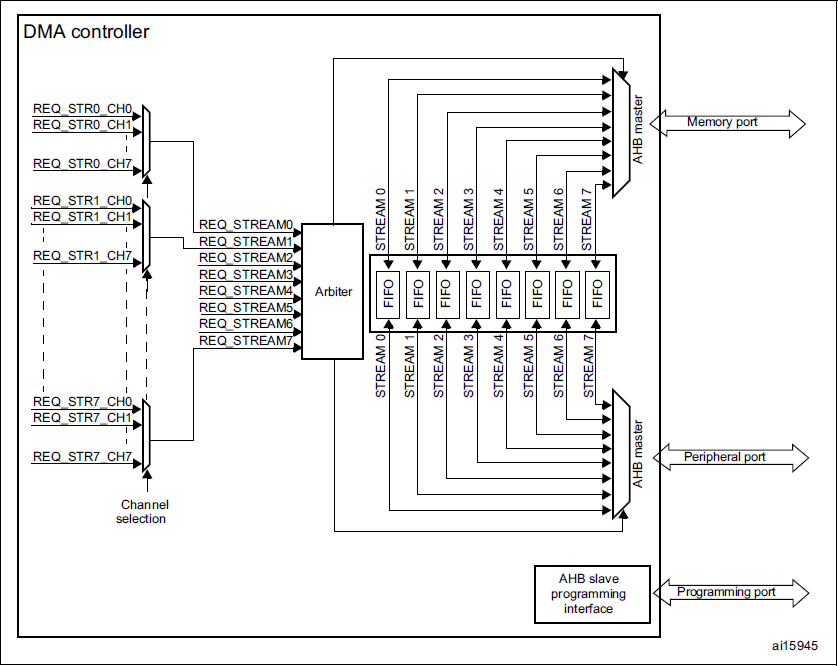
\includegraphics[height=10 cm]{f407_dma_block_diagram.png}
	\caption{Blok dijagram DMA kontrolera na STM32F407VGT6 mikrokontroleru \cite{f407_manual}}
	\label{fig:f407_dma_block_diagram}
\end{figure}

DMA kontroler obavlja izravan prijenos memorije; kao AHB (engl. \textit{AMBA High-performance Bus}, AMBA na engl. \textit{Advanced Microcontroler Bus Architecture}) \textit{master}, može u bilo kojem trenutku preuzeti kontrolu nad AHB sabirnicom i pokrenuti AHB transakcije. DMA kontroler može pokrenuti sljedeće transakcije:
\begin{itemize}
	\item prijenos sa periferije na memoriju,
	\item prijenos sa memorije na periferiju,
	\item prijenos sa memorije na memoriju.
\end{itemize}
S obzirom na to da se u ovom radu koriste prijenosi s periferije na memoriju i obrnuto, u daljnjem tekstu će se podrazumijevati samo ti slučajevi.

DMA periferija ima dvije AHB \textit{master} sabirnice, jedna se koristi za pristup memoriji, a druga za pristup periferijama. AHB \textit{slave} sabirnica se koristi za programiranje DMA kontrolera.

Pojedini kontroler ima 8 tokova (engl. \textit{stream}), te za svaki tok postoji 8 kanala (engl. \textit{channel}). Svaki tok je spojen na određeni sklopovski DMA kanal. Tokovi i kanali služe kako bi se ostvarila veza između ostalih periferija i DMA mikokrontrolera, tako da periferije mogu slati zahtjev za DMA prijenos. %Broj podataka koji se trebaju prenijeti (do 65535) je programabilan i povezan je sa širinom izvora periferije koja zahtijeva DMA prijenos. Registar koji sadržava broj podataka koji se trebaju prenijeti se dekrementira nakon svake transakcije.

Svaki DMA prijenos se sastoji od tri operacije:
\begin{itemize}
	\item učitavanje sa periferijskog podatkovnog registra ili lokacije u memoriji, čije su adrese zapisane u DMA\_SxPAR ili DMA\_SxM0AR registru
	\item spremanje podataka na periferijski podatkovni registar ili lokaciju u memoriji, čije su adrese zapisane u DMA\_SxPAR ili DMA\_SxM0AR registru
	\item naknadno dekrementiranje DMA\_SxNDTR registra, koji sadržava broj podataka koji se još trebaju prenjeti
\end{itemize}
Spomenuti registri su prikazani u tablici \ref{Tab:f407_dma_register_map_1}. Kada periferija želi pristupiti DMA kontroleru, periferijski sklop šalje zahtjev DMA kontroleru. DMA kontroler poslužuje zahtjev ovisno o prioritetima kanala. Čim DMA kontroler pristupi periferiji, DMA kontroler periferiji šalje signal potvrde. Periferni uređaj ukida svoj zahtjev čim dobije potvrdni signal iz DMA kontrolera. Nakon što periferna jedinica ukine zahtjev, DMA kontroler ukida signal potvrde. Ako ima više zahtjeva, periferna jedinica može pokrenuti sljedeću transakciju.

\begin{table}[H]
	\caption{Registri DMA\_SxPAR, DMA\_SxM0AR i DMA\_SxNDTR kod STM32F407VGT6 mikrokontrolera. \textit{x} označava broj toka \cite{f407_manual}}
	\resizebox{\textwidth}{!}{%
	\begin{tabular}{|c|c|l|l|l|l|l|l|l|l|l|l|l|l|l|l|l|l|l|l|l|l|l|l|l|l|l|l|l|l|l|l|l|}
		\hline
		\textbf{\begin{tabular}[c]{@{}c@{}}Register\\ name\end{tabular}} & \rotbf{31} & \rotbf{30} & \rotbf{29} & \rotbf{28} & \rotbf{27} & \rotbf{26} & \rotbf{25} & \rotbf{24} & \rotbf{23} & \rotbf{22} & \rotbf{21} & \rotbf{20} & \rotbf{19} & \rotbf{18} & \rotbf{17} & \rotbf{16} & \rotbf{15} & \rotbf{14} & \rotbf{13} & \rotbf{12} & \rotbf{11} & \rotbf{10} & \rotbf{9} & \rotbf{8} & \rotbf{7} & \rotbf{6} & \rotbf{5} & \rotbf{4} & \rotbf{3} & \rotbf{2} & \rotbf{1} & \rotbf{0} \\
		\hline
		DMA\_SxPAR & \multicolumn{32}{c|}{PA[31:0]} \\
		\hline
		Reset value & 0 & 0 & 0 & 0 & 0 & 0 & 0 & 0 & 0 & 0 & 0 & 0 & 0 & 0 & 0 & 0 & 0 & 0 & 0 & 0 & 0 & 0 & 0 & 0 & 0 & 0 & 0 & 0 & 0 & 0 & 0 & 0 \\
		\hline
		DMA\_M0AR & \multicolumn{32}{c|}{M0A[31:0]} \\
		\hline
		Reset value & 0 & 0 & 0 & 0 & 0 & 0 & 0 & 0 & 0 & 0 & 0 & 0 & 0 & 0 & 0 & 0 & 0 & 0 & 0 & 0 & 0 & 0 & 0 & 0 & 0 & 0 & 0 & 0 & 0 & 0 & 0 & 0 \\
		\hline
		DMA\_SxNDTR & \multicolumn{16}{c|}{Res.} & \multicolumn{16}{c|}{NDT[15:0]}\\
		\hline
		Reset value & & & & & & & & & & & & & & & & & 0 & 0 & 0 & 0 & 0 & 0 & 0 & 0 & 0 & 0 & 0 & 0 & 0 & 0 & 0 & 0 \\
		\hline
	\end{tabular}%
	}
	\label{Tab:f407_dma_register_map_1}
\end{table}

Svaki tok je povezan sa DMA zahtjevom, koji može biti odabran između 8 mogućih kanalnih zahtjeva. Odabir kanala određuju bitovi CHSEL[2:0] u DMA\_SxCR registru (tablica \ref{Tab:f407_dma_register_map_2}). Odabir kanala prikazan je na slici \ref{fig:f407_dma_channel_selection}.
\begin{table}[H]
	\caption{Registar DMA\_SxCR kod STM32F407VGT6 mikrokontrolera \citep{f407_manual}}
	\resizebox{\textwidth}{!}{%
	\begin{tabular}{|c|c|l|l|l|l|l|l|l|l|l|l|l|l|l|l|l|l|l|l|l|l|l|l|l|l|l|l|l|l|l|l|l|}
		\hline
		\textbf{\begin{tabular}[c]{@{}c@{}}Register\\ name\end{tabular}} & \rotbf{31} & \rotbf{30} & \rotbf{29} & \rotbf{28} & \rotbf{27} & \rotbf{26} & \rotbf{25} & \rotbf{24} & \rotbf{23} & \rotbf{22} & \rotbf{21} & \rotbf{20} & \rotbf{19} & \rotbf{18} & \rotbf{17} & \rotbf{16} & \rotbf{15} & \rotbf{14} & \rotbf{13} & \rotbf{12} & \rotbf{11} & \rotbf{10} & \rotbf{9} & \rotbf{8} & \rotbf{7} & \rotbf{6} & \rotbf{5} & \rotbf{4} & \rotbf{3} & \rotbf{2} & \rotbf{1} & \rotbf{0} \\
		\hline
		DMA\_SxPAR & \multicolumn{4}{c|}{Res.} & \multicolumn{3}{c|}{\rot{CHSEL[2:0]}} & \multicolumn{2}{c|}{\rot{MBURST[1:0]}} & \multicolumn{2}{c|}{\rot{PBURST[1:0]}} & \rot{Res.} & \rot{CT} & \rot{DBM} & \multicolumn{2}{c|}{\rot{PL[1:0]}} & \rot{PINCOS} & \multicolumn{2}{c|}{\rot{MSIZE[1:0]}} & \multicolumn{2}{c|}{\rot{PSIZE[1:0]}} & \rot{MINC} & \rot{PINC} & \rot{CIRC} & \multicolumn{2}{c|}{\rot{DIR[1:0]}} & \rot{PFCTRL} & \rot{TCIE} & \rot{HTIE} & \rot{TEIE} & \rot{DMEIE} & \rot{EN} \\
		\hline
		Reset value & & & & & 0 & 0 & 0 & 0 & 0 & 0 & 0 & & 0 & 0 & 0 & 0 & 0 & 0 & 0 & 0 & 0 & 0 & 0 & 0 & 0 & 0 & 0 & 0 & 0 & 0 & 0 & 0 \\
		\hline
	\end{tabular}%
	}
	\label{Tab:f407_dma_register_map_2}
\end{table} 
\begin{figure}[H]
	\centering
	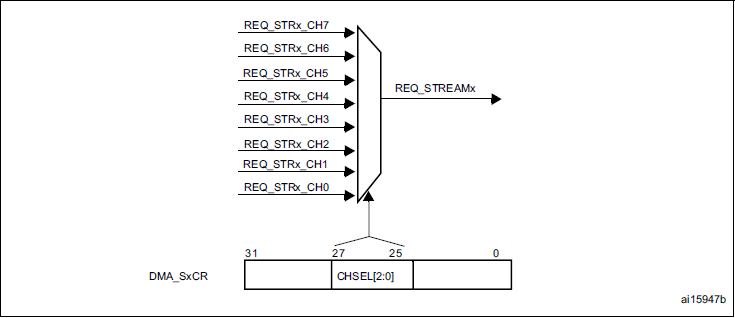
\includegraphics[width=\textwidth]{f407_dma_channel_selection.png}
	\caption{Odabir kanala \citep{f407_manual}}
	\label{fig:f407_dma_channel_selection}
\end{figure}
Proučavanjem dokumentacije mikrokontrolera, zaključeno je da je za SPI prijenos putem DMA sklopa potrebno koristiti kanal 0 i tokove 3 (SPI2\_RX) i 4 (SPI2\_TX) \cite[str. 307]{f407_manual}. Odabrani tokovi se koriste zato što je kamera spojena na SPI2 periferiju mikrokontrolera.

Blok dijagram DMA periferije na STM32L471VGT6 mikrokontroleru je prikazan na slici \ref{fig:l471_dma_block_diagram}. Vidljivo je da oba mikrokontrolera sadržavaju dvije DMA periferije. Za razliku od SMT32F407VGT6 mikrokontrolera, trenutačni mikrokontroler, STM32L471VGT6, nema dvije AHB \textit{master} sabirnice, već samo jednu AHB \textit{master} sabirnicu.

STM32L471VGT6 nema tokove za ostvarivanje veze između periferija i DMA sklopa, već ima samo kanale, te se stoga veza između ostalih periferija i DMA kontrolera ostvaruje na drugačiji način, prikazan na slici \ref{fig:l471_dma_request_mapping}. Iz slike je vidljivo da se na ovom mikrokontroleru trebaju koristiti kanali 4 (SPI2\_RX) i 5 (SPI2\_TX).

Još jedna razlika između DMA periferija dvaju mikrokontrolera se krije u prekidima koje DMA kontrolera i zastavicama za prekide. STM32F407VGT6 ima 5 različitih prekida: završetak prijenosa (TC, engl. \textit{Transfer Complete}), obavljena polovica prijenosa (HT, engl. \textit{Half Transfer}), greška u prijenosu (TE, engl. \textit{Transfer Error}), FIFO greška (FE, engl. \textit{FIFO Error}) i greška u direktnom načinu rada (DME, engl. \textit{Direct Mode Error}). STM32L471VGT6 ima 3 različita prekida: završetak prijenosa završetak prijenosa (TC), obavljena polovica prijenosa (HT), greška u prijenosu (TE). Kod STM32L471VGT6 postoji još globalni prekid (GI, engl. \textit{Global Interrupt}) koji se aktivira u svim slučajevima. Ako se, na primjer, želi DMA kontroler namjestiti da zahtijeva prekid kod završetka prijenosa, polovice prijenos i kod greške u prijenosu, to se može podesiti jednostavno aktiviranjem globalnih prekida. S obzirom na to STM32F407VGT6 sadržava više vrsta prekida, on sadržava i 2 prekidna registra, dok STM32L471VGT6 sadržava 1 prekidni registar.

\begin{figure}[H]
	\centering
	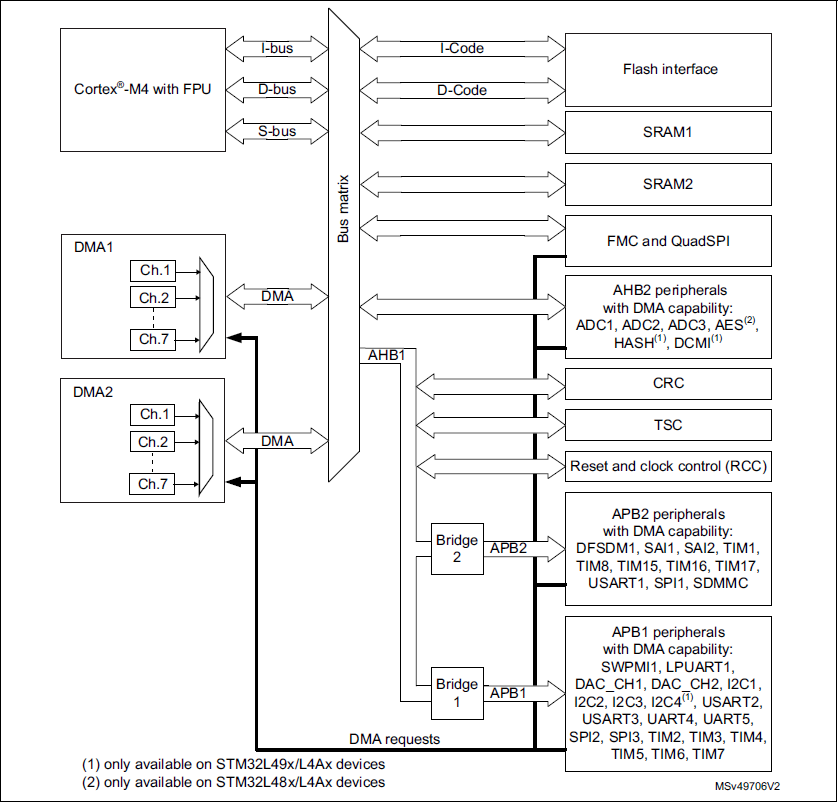
\includegraphics[width=\textwidth]{l471_dma_block_diagram.png}
	\caption{Blok dijagram DMA periferije na STM32L471VGT6 mikrokontroleru \cite{l471_manual}}
	\label{fig:l471_dma_block_diagram}
\end{figure}

\begin{figure}[H]
	\centering
	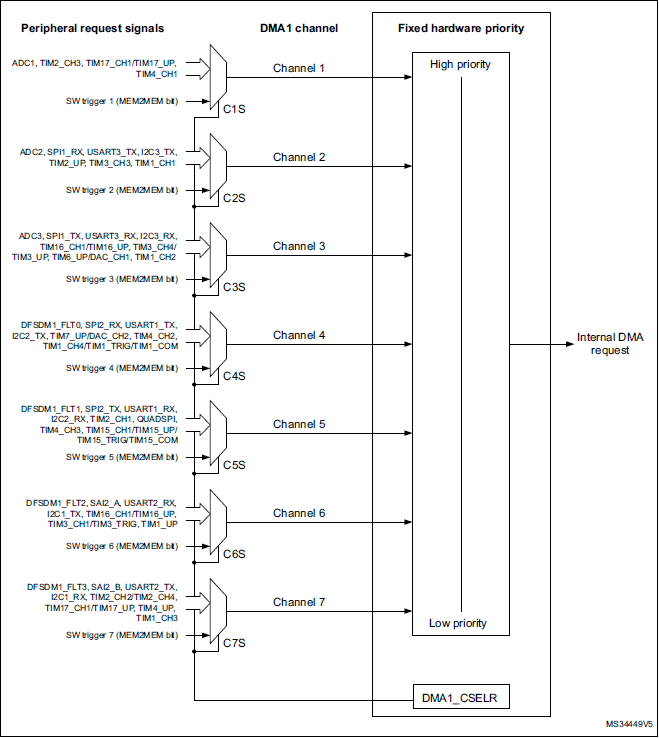
\includegraphics[width=10 cm]{l471_dma_request_mapping.png}
	\caption{Mapiranje zahtjeva za DMA1 kontroler kod STM32L471VGT6 mikrokontrolera \cite[str. 338]{l471_manual}}
	\label{fig:l471_dma_request_mapping}
\end{figure}

Što se tiče ostalih dijelova DMA periferija, mikrokontroleri funkcioniraju isto. Postoje, međutim, razlike u načinu konfiguracije DMA kontrolera, međutim, to nije predstavljalo problem, s obzirom na to da je konfiguracija prepuštena generatoru koda. Nazivi registara koji se koriste su također različiti između dva mikrokontrolera, iako su im funkcije iste. To također nije bio problem jer su se koristile definicije registara u programskoj podršci koju je pružao proizvođač mikrokontrolera, pa je bilo potrebno samo promijeniti nazive tih registara.

\section{CAN protokol}

S obzirom na to da je na tiskanoj pločici PDH sustava sklopovlje za CAN komunikaciju krivo povezan, nije bilo moguće napisati programsku podršku za CAN komunikaciju. Međutim, u ovom poglavlju dati će se opis protokola, kao i njegova implementacija na mikrokontroleru, te će se izložiti mogućnosti implementacije u ovaj projekt.

\subsection{Opis protokola}

CAN je serijska komunikacijska sabirnica koju je standardizirao ISO (engl. \textit{International Standardization Organization}), a razvijena je od strane tvrtke BOSCH za automobilsku industriju s ciljem da se zamijeni složeni žičani kabel s dvožičnom sabirnicom \cite{can_manual}. Specifikacija zahtijeva su visoka otpornost na električne smetnje i sposobnost otkrivanja i ispravljanja greški kod prijenosa podataka.

Komunikacijski protokol CAN opisuje kako se informacija prenosi između uređaja na mreži i kako odgovara OSI (engl. \textit{Open Systems Interconnection}) modelu koji je definiran u slojevima (slika \ref{fig:can_osi_model}). Stvarna komunikacija između uređaja spojenih fizičkim medijem je definirana fizičkim slojem modela.

\begin{figure}[H]
	\centering
	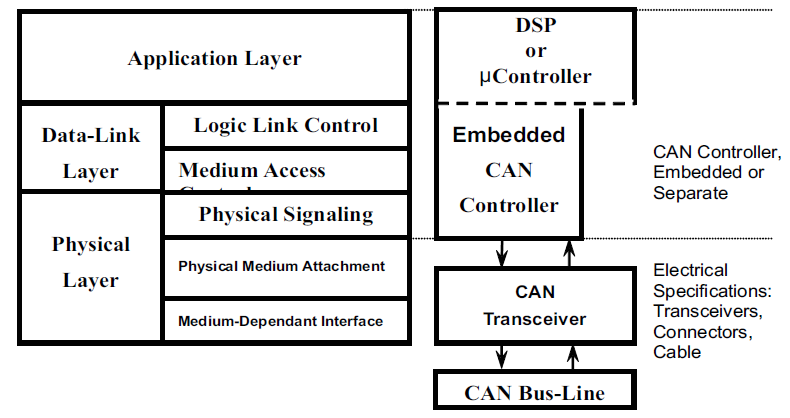
\includegraphics[width=\textwidth]{can_osi_model.png}
	\caption{OSI model CAN protokola \cite[str. 2]{can_manual}}
	\label{fig:can_osi_model}
\end{figure}

CAN komunikacijski protokol je protokol s višestrukim pristupom, osluškivanjem nosioca, detekcijom sudara i arbitražom na paritet poruka (CSMA/CD+AMP). CSMA znači da svaki čvor na sabirnici mora čekati određeni period neaktivnosti prije nego što pokuša poslati poruku. CD+AMP znači da se sudari rješavaju bitovnom (\textit{bit-wise}) arbitražom, koja se temelji na prethodno namještenom prioritetu svake poruke u identifikacijskom polju poruke. Viši prioritet uvijek dobiva pristup sabirnici.

Standardni CAN protokol s identifikatorom širine 11 bita omogućava brzine prijenosa od 125 kb/s do 1 Mb/s. Standardni protokol u praktičnim primjenama je zamijenjen s proširenim protokolom s identifikatorom širine 29 bita. Standardni 11-bitni identifikator omogućava 2\textsuperscript{11}, ili 2048 različitih identifikatora poruka, dok prošireni 29-bitni identifikator omogućava 2\textsuperscript{29}, ili 536870912 različitih identifikatora. 

\subsubsection{Standardni CAN protokol}

Standardni CAN sa 11-bitnim identifikatorom je prikazan na slici \ref{fig:standard_can_bits}.
\begin{figure}[H]
	\centering
	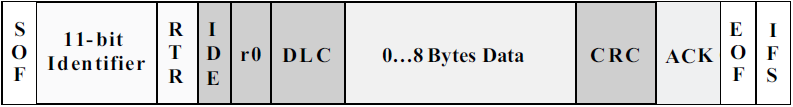
\includegraphics[width=\textwidth]{standard_can_bits.png}
	\caption{Standardna CAN poruka: 11-bitni identifikator \cite[str. 3]{can_manual}}
	\label{fig:standard_can_bits}
\end{figure}
Značenje pojedinih bitova na slici \ref{fig:standard_can_bits} su:
\begin{itemize}
	\item SOF - jedan bit, početak okvira (engl. \textit{Start Of Frame}), označava početak poruke i koristi se za sinkronizaciju čvorova na sabirnici nakon mirovanja,
	\item Identifikator - 11-bitni identifikator standardnog CAN protokola, uspostavlja prioritet poruke. Manja binarna vrijednost znači viši prioritet,
	\item RTR - jedan bit, zahtjev za udaljenim prijenosom (engl. \textit{Remote Transmission Request}) dominantan je kada se traži informacija s drugog čvora. Svi čvorovi prime zahtjev, ali identifikator određuje traženi čvor. Povratna informacija se također šalje na sve čvorove i svaki čvor ju može iskoristiti ako je potrebno. Na taj su način svi podatci koji se koriste u sustavu uniformni,
	\item IDE - jedan bit, proširenje identifikatora (engl. \textit{Identifier Extension}), označava da se šalje standardni CAN identifikator bez proširenja,
	\item r0 - rezervirani bit (za moguću upotrebu kod budućih dopuna standarda),
	\item DLC - 4-bitna širina podatkovnog koda (engl. \textit{Data Length Code}), sadržava broj bajtova podatka koji se šalje,
	\item Podatci - može se slati do 64 bitova aplikacijskih podataka,
	\item CRC - 16-bitna (15 bitova plus granični bit) ciklička provjera redundancije (engl. \textit{Cyclic Redundancy Check}) sadržava kontrolni zbroj (\textit{checksum}, broj poslanih bitova) prethodnih aplikacijskih podataka za detekciju grešaka,
	\item ACK - svaki čvor koji primi točnu poruku prepisuje ovaj recesivni bit u izvornoj poruci s dominantnim bitom, što znači da je poslana poruka bez greške. Ako prijemni čvor otkrije pogrešku i ostavi ovaj bit recesivnim, on odbacuje poruku i čvor koji šalje poruku ponavlja poruku nakon rearbitraže. Tako svaki čvor priznaje (ACK) integritet svojih podataka. ACK sadrži 2 bita, jedan je bit potvrde, a drugi je graničnik,
	\item EOF - 7-bitno polje, kraj okvira (engl. \textit{End Of Frame}), označava kraj poruke i onemogućuje trpanje bitova, ukazujući na grešku kod trpanja u slučaju da je dominantan. Kada 5 bitova iste logičke razine nastanu u slijedu kod normalne operacije, bit suprotne logičke razine se \textit{natrpa} u podatke,
	\item IFS - 7-bitno polje, međuokvirni prostor (engl. \textit{Interframe Space}), sadržava vrijeme potrebno da kontroler pomakne ispravno primljen okvir na njegovu valjanu poziciju u međuspremniku poruka.
\end{itemize}

\subsubsection{Prošireni CAN protokol}

\begin{figure}[H]
	\centering
	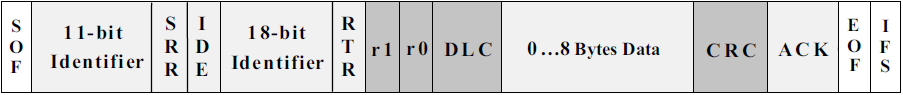
\includegraphics[width=\textwidth]{extended_can_bits.png}
	\caption{Proširena CAN poruka: 29-bitni identifikator \cite[str. 4]{can_manual}}
	\label{fig:extended_can_bits}
\end{figure}
Na slici \ref{fig:extended_can_bits} je vidljivo da je proširena CAN poruka ista kao i standardna, uz dodatak:
\begin{itemize}
	\item SRR - zamjenski udaljeni pristup (engl. \textit{Substitute Remote Request}), zamjenjuje RTR bit u standardnoj poruci kao rezervirano mjesto u proširenom formatu,
	\item IDE - recesivni bit u proširenju identifikatora (engl. \textit{Identifier Extension} označava da slijedi još identifikatorskih bitova. 18-bitno proširenje slijedi nakon IDE,
	\item r1 - nakon RTR i r0 bitova, dodan je još jedan rezervirani bit prije DLC bita.
\end{itemize}

\subsubsection{CAN poruka}

\paragraph{Arbitraža}

Temeljna karakteristika CAN protokola je suprotno logičko stanje između sabirnice, upravljačkog ulaza i izlaza prijamnika (slika \ref{fig:inverted_logic_can}). U općenitom slučaju visoka logička razina se poistovjećuje s jedinicom, a niska logička razina se poistovjećuje s nulom, međutim, tako nije na CAN sabirnici. Pristup sabirnici se događa nasumično. Ako dva čvora pokušavaju istovremeno zauzeti sabirnicu, pristup se omogućuje pomoću nedestruktivne bitovne arbitraže. Nedestruktivno znači da postupak arbitraže ni na koji način ne utječe na poruke, odnosno čvor koji dobije arbitražu može nastaviti sa slanjem poruke.

\begin{figure}[H]
	\centering
	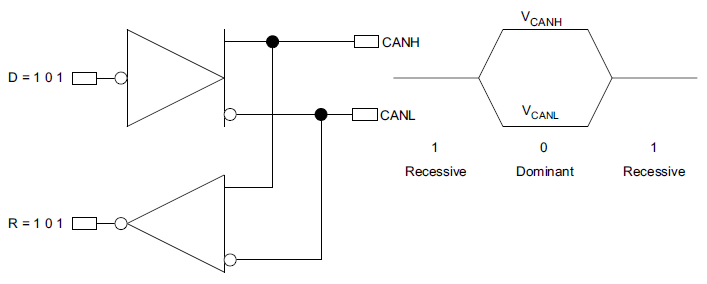
\includegraphics[width=\textwidth]{inverted_logic_can.png}
	\caption{Obrnuta logika CAN sabirnice \cite[str. 4]{can_manual}. D je upravljački ulaz, a R je izlaz prijamnika}
	\label{fig:inverted_logic_can}
\end{figure}

Alokacija prioriteta porukama u identifikatoru je svojstvo CAN protokola koje ga čini pogodnim za upotrebu u sustavima za rad u stvarnom vremenu. Što je binarni broj identifikatora poruke niži, to je prioritet poruke viši. Identifikator koji se u potpunosti sastoji od nula čini poruku najvišeg prioriteta na mreži jer zadržava sabirnicu dominantnom najdulje. Iz tog razloga, ako dva čvora počnu sa slanjem poruke istovremeno, čvor koji pošalje posljednji identifikatorski bit kao nulu (dominantan) dok drugi čvor pošalje jedinicu (recesivan) zadržava kontrolu nad CAN sabirnicom i nastavlja sa slanjem poruke. Dominantan bit uvijek prebriše recesivan bit na CAN sabirnici.

Treba imati na umu da čvor koji šalje poruku stalno nadzire svaki bit svog prijenosa. Ovo je razlog za konfiguraciju primopredajnika na slici \ref{fig:inverted_logic_can} u kojoj su CANH i CANL izlazne stezaljke upravljačkog sklopa interno povezane s ulazom prijemnika. Kašnjenje radi propagacije signala u unutarnjoj petlji od upravljačkog ulaza do izlaza prijemnika se obično koristi kao kvalitativna mjera CAN primopredajnika. Ovo propagacijsko kašnjenje se naziva vrijeme petlje (engl. \textit{loop time}).

Slika \ref{fig:can_arbitration} prikazuje proces arbitraže kojim CAN kontroler automatski upravlja. Budući da svaki čvor kontinuirano nadzire vlastiti prijenos, dok dominantni bit čvora C prebrisuje recesivni bit čvora B, čvor B detektira da se stanje sabirnice ne poklapa sa bitom koji je poslao. Posljedično, čvor B prestaje sa prijenosom dok čvor C nastavlja sa slanjem poruke. Čvor B ponovno pokušava pristupiti sabirnici nakon što čvor C otpusti sabirnicu.

\begin{figure}[H]
	\centering
	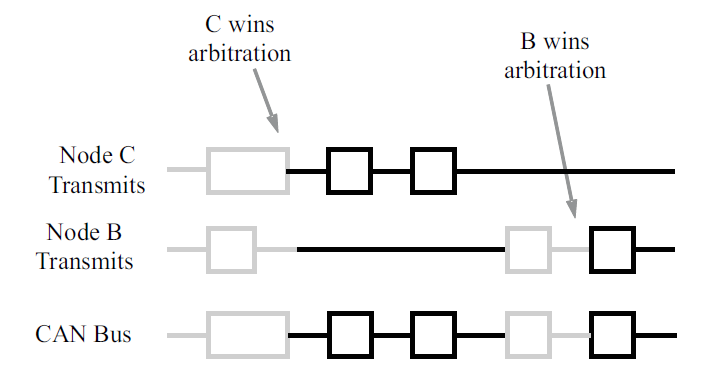
\includegraphics[width=\textwidth]{can_arbitration.png}
	\caption{Arbitraža na CAN sabirnici \cite[str. 5]{can_manual}}
	\label{fig:can_arbitration}
\end{figure}

\paragraph{Tipovi CAN poruka}

Postoje četiri tipova poruka, odnosno okvira, a to su:
\begin{itemize}
	\item Podatkovni okvir - najčešći oblik poruka, sastoji se od arbitražnog polja, podatkovnog polja, CRC polja, i potvrdnog polja. Arbitražno polje se sastoji od 11-bitnog identifikatora na slici \ref{fig:standard_can_bits} i RTR bita, koji je dominantan za podatkovne okvire. Na slici \ref{fig:extended_can_bits} sadržava 29 bitova i RTR bit. Slijedi podatkovno polje koje sadržava od 0 do 8 bajtova podataka, a zatim slijedi CRC polje koje sadržava 16-bitni kontrolni zbroj koji se koristi za detekciju pogrešaka. Potvrdno polje je posljednje,
	\item Daljinski okvir - svrha daljinskog okvira je traženje prijenosa podataka s drugog čvora. Daljinski okvir sličan je podatkovnom okviru, s dvije važne razlike. Prvo, ovaj tip poruke je eksplicitno označen kao daljinski okvir preko recesivnog RTR bita u arbitražnom polju, a druga razlika je da nema podataka,
	\item Okvir pogreške - ovo je posebna poruka koja krši pravila formata CAN poruke. Odašilje ju čvor kada detektira pogrešku u poruci, i uzrokuje da svi ostali čvorovi u mreži počnu slati okvir pogreške. Izvorni odašiljač zatim automatski ponovno pošalje poruku. Sustav brojača pogrešaka u CAN kontroleru osigurava da čvor ne zauzima sabirnicu uzastopnim slanjem okvira pogreške,
	\item Okvir preopterećenja - okvir preopterećenja se spominje radi cjelovitosti. Sličan je okviru pogreške u smislu formata i odašilje ga čvor koji postane previše zauzet. Primarno se koristi kao dodatna odgoda između poruka.
\end{itemize}

\paragraph{Ispravan okvir}

Kada je posljednji bit završnog EOF polja primljen bez grešaka u recesivnom stanju, smatra se da je poruka bez greške. Dominantan bit u EOF polju uzrokuje da odašiljač ponovi slanje.

\subsubsection{Provjera pogrešaka i ograničenje grešaka}

Robusnost CAN protokola može se djelomično pripisati njegovim brojnim postupcima provjere pogrešaka. CAN protokol uključuje pet metoda provjere grešaka: tri na razini poruke i dvije na razini bita. Ako poruka ne uspije proći na bilo kojoj od ovih metoda otkrivanja pogreške, ona se ne prihvaća, te prijemni čvor generira okvir pogreške. Ovime se prisiljava odašiljački čvor da ponovno pošalje poruku dok se ne primi ispravna poruka. Ako neispravni čvor prekine sabirnicu kontinuiranim ponavljanjem pogreške, njegov kontroler uklanja sposobnost prijenosa nakon što se dosegne ograničenje broja pogrešaka.

Provjeru pogreške na razini poruke provode CRC i ACK bitovi prikazani na slikama \ref{fig:standard_can_bits} i \ref{fig:extended_can_bits}. 16-bitni CRC sadrži kontrolni zbroj podataka prethodne aplikacije za otkrivanje pogreške s 15-bitnim kontrolnim zbrojem i 1-bitnim graničnikom. Polje ACK je dugo dva bita i sastoji se od bita potvrde i graničnog bita.

Na razini poruke provodi se također i provjera formata. Ova provjera pretražuje polja u poruci koja uvijek moraju sadržavati recesivne bitove. Ako se detektira dominantan bit, stvara se pogreška. Bitovi koji se provjeravaju su SOF, EOF, ACK granični bit i CRC granični bit.

Na razini bita svaki odaslani bit nadzire odašiljač poruke. Ako je podatkovni bit (ne arbitražni bit) zapisan na sabirnicu, a pročitan je suprotan bit, generira se pogreška. Jedine iznimke su kod identifikatorskog polja poruke koja se koriste kod arbitraže i potvrdno polje koje zahtjeva da recesivni bit bude prebrisan od strane dominantnog bita.

Posljednja metoda detekcije pogreške je pravilo umetanja redundantnih bitova \\ \engl{bit stuffing}, gdje nakon pet uzastopnih bitova iste logičke razine, ako sljedeći bit nije komplement, generira se pogreška. Umetanje redundantnih bitova osigurava dostupnost rastućih bridova za tekuću sinkronizaciju mreže. Umetanje također osigurava da se tok bitova ne zamijeni s okvirom pogreške ili 7-bitnim međuokvirnim prostorom koji predstavlja kraj poruke. Umetnute bitove miče kontroler prijemnog čvora prije nego se podatci proslijede aplikaciji. S ovom logikom, aktivni okvir pogreške sastoji se od šest bitova, što krši pravilo umetanja redundantnih bitova. Ovo se tumači kao pogreška od strane svih CAN čvorova koji zatim generiraju vlastiti okvir pogreške. To znači da okvir pogreške može biti dugačak od originalnih šest do dvanaest bitova sa svim odgovorima. Nakon ovog okvira pogreške slijedi polje razgraničenja od osam recesivnih bitova i razdoblje mirovanja sabirnice prije ponovnog slanja oštećene poruke. Važno je napomenuti da ponovno poslana poruka još uvijek mora proći arbitražu kako bi dobila pristup sabirnici.

\subsubsection{CAN sabirnica}

Podatkovna veza i slojevi fizičke signalizacije na slici \ref{fig:can_osi_model}, koji su inače transparentni operateru sustava, uključeni su u svaki kontroler koji implementira CAN protokol. Veza s fizičkim medijem se onda implementira kroz linijski primopredajnik kako bi se formirao sistemski čvor prikazan na slici \ref{fig:can_bus_details}.
\begin{figure}[H]
	\centering
	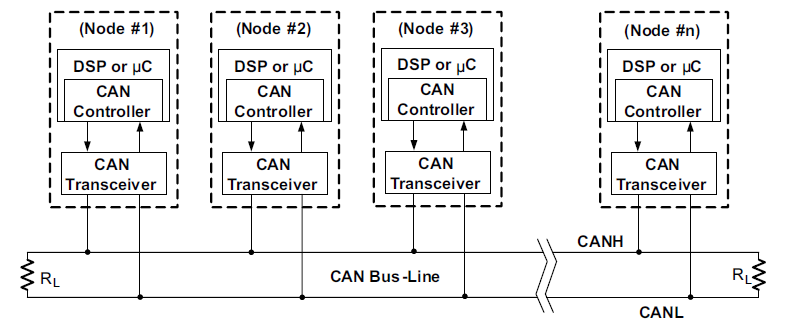
\includegraphics[width=\textwidth]{can_bus_details.png}
	\caption{Detalji CAN sabirnice \cite[str. 7]{can_manual}}
	\label{fig:can_bus_details}
\end{figure}
Signalizacija je diferencijalna, odakle CAN dobiva svoju robusnu otpornost na šum i toleranciju na pogreške. Uravnoteženo diferencijalno signaliziranje smanjuje šum i dopušta visoku brzinu signalizacije preko kabela s upletenom paricom. Uravnoteženo znači da je tok struje u svakoj signalnoj liniji jednak, ali suprotan po smjeru, što rezultira efektom poništavanja polja, što je ključno za niske emisije šuma.

Specifikacije standarda visoke brzine ISO 11898 dane su za maksimalnu brzinu prijenosa 1 Mbps s duljinom sabirnice od 40 m, s najviše 30 čvorova. Preporučuje se da se linije terminiraju na oba kraja s otpornicima R\textsubscript{L}, koji odgovaraju karakterističnoj impedanciji linije kako bi se spriječila refleksija signala.

Izgled recesivnih i dominantnih bitova na signalnim linijama CANH i CANL prikazan je na slici \ref{fig:can_bus_states}.
\begin{figure}[H]
	\centering
	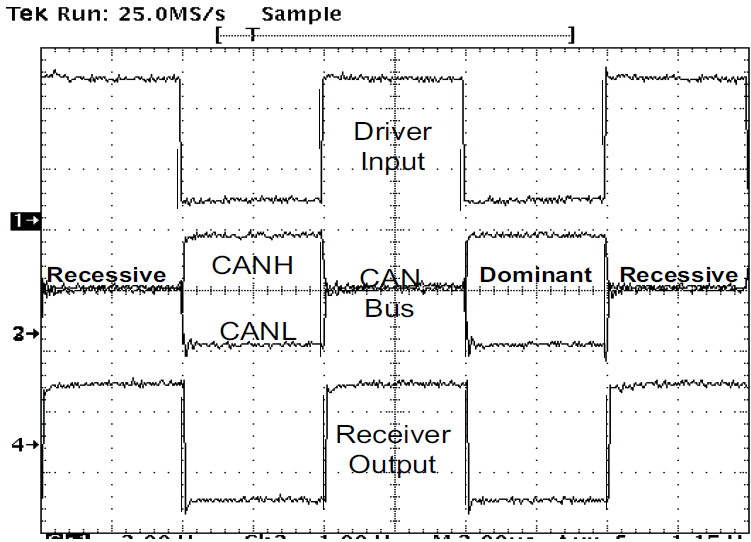
\includegraphics[height=7 cm]{can_bus_states.png}
	\caption{Dominantno i recesivno stanje na CAN sabirnici \cite[str. 8]{can_manual}}
	\label{fig:can_bus_states}
\end{figure}

CAN standard definira komunikacijsku mrežu koja povezuje sve čvorove spojene na sabirnicu i omogućava im međusobnu komunikaciju. Može, ali ne mora postojati središnji kontrolni čvor, a čvorovi se mogu dodavati u bilo kojem trenutku, čak i kad se na mreži odvija komunikacija \engl{hot-plugging}.

Primjer komunikacije između tri čvora dan je na slici \ref{fig:can_bus_traffic}. Čvor A završi slanje svoje poruke kada čvorovi B i C potvrde primitak ispravne poruke. Čvorovi B i C zatim započnu arbitražu, čvor C dobiva arbitražu i pošalje svoju poruku. Čvorovi A i B potvrde primitak poruke čvora C, te zatim čvor B nastavi sa slanjem svoje poruke. Obratiti pažnju na suprotni polaritet upravljačkog ulaza i izlaza na sabirnici.
\begin{figure}[H]
	\centering
	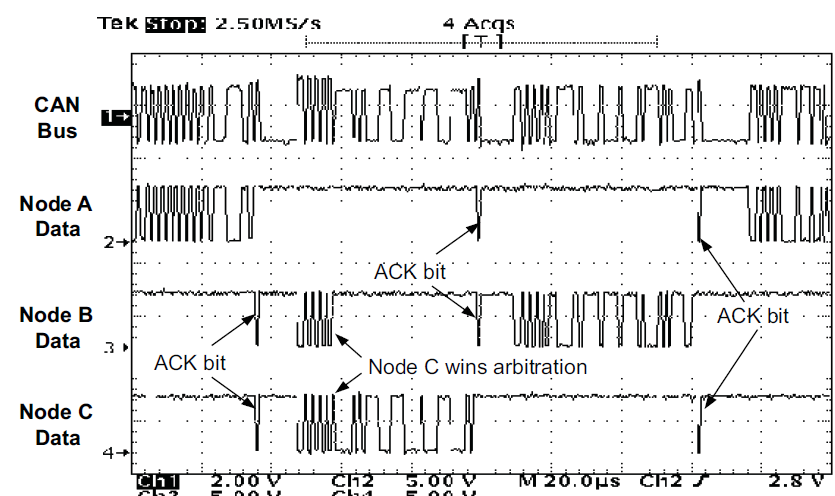
\includegraphics[height=7 cm]{can_bus_traffic.png}
	\caption{Promet na CAN sabirnici \cite[str. 9]{can_manual}}
	\label{fig:can_bus_traffic}
\end{figure}

\subsection{CAN periferijsko sklopovlje na STM32L471VGT6 mikrokontroleru}

CAN periferija kod STM32L471VGT6 mikrokontrolera se naziva bxCAN \engl{Basic Extended CAN}. Podržava CAN protokole verzije 2.0A i B. Osim aplikacijskih poruka dodane su još i dijagnostičke poruke i poruke za upravljanje mrežom. Blok dijagram CAN periferijskog sklopovlja prikazan je na slici \ref{fig:can_block_diagram}.
\begin{figure}[H]
	\centering
	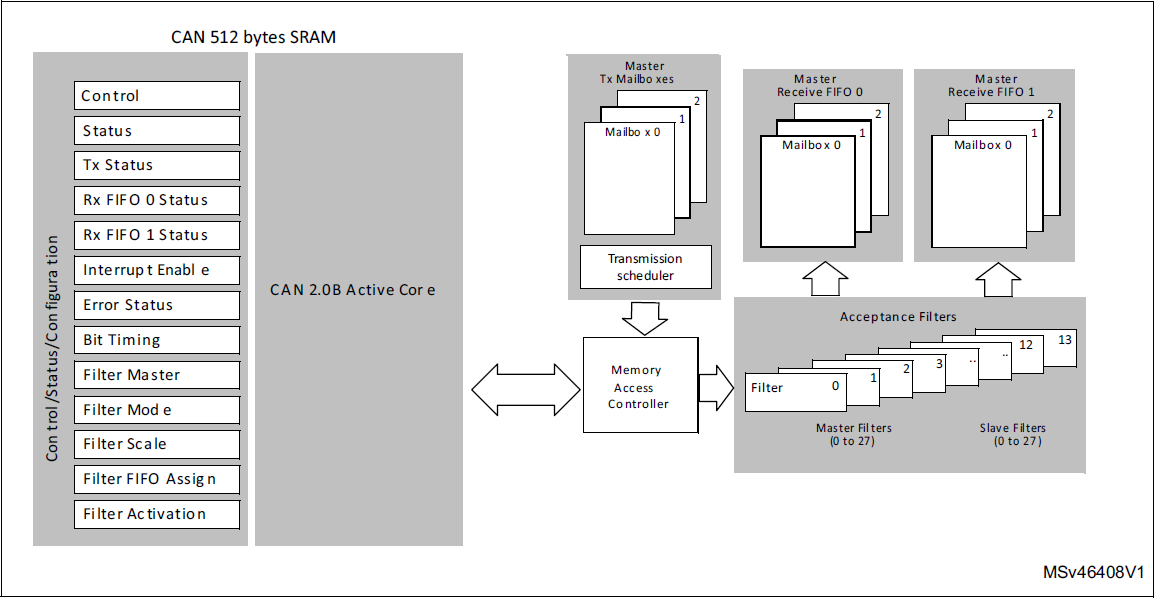
\includegraphics[width=\textwidth]{can_block_diagram.png}
	\caption{Blok dijagram CAN periferije na STM32L471VGT6 mikrokontroleru}
	\label{fig:can_block_diagram}
\end{figure}
Modul bxCAN rukuje s prijenosom CAN poruka potpunosti automatski. Sklopovlje podržava standardne (11-bitne) i proširene (29-bitne) identifikatore. Aplikacija koristi kontrolne, statusne i konfiguracijske registre kako bi:
\begin{itemize}
	\item konfigurirala CAN parametre, npr. baud rate,
	\item zahtijevala slanja,
	\item rukovala prijemima,
	\item upravljala prekidima,
	\item dobivala dijagnostičke podatke.
\end{itemize}
Za postavljanje poruka, programska podrška na raspolaganju ima tri odašiljačke \textit{mailbox} strukture. Planer slanja odlučuje koja \textit{mailbox} struktura će se prvo slati. bxCAN pruža do 14 skalabilnih/podesivih banaka filtara za odabir nadolazećih poruka koje programska podrška treba, a ostale odbacuje. Sklopovlje koristi dvije primajuće FIFO \engl{First Input First Output} strukture za spremanje poruka. FIFO znači da se prvi podatak koji se unese prvi obrađuje. Tri kompletne poruke se mogu pohraniti u svaku FIFO strukturu. Sklopovlje u potpunosti upravlja FIFO strukturama.

\subsubsection{Načini rada bxCAN sklopovlja}

Sklopovlje bxCAN može raditi u tri glavna načina rada, a to su inicijalizacijski, normalni i spavajući. Nakon sklopovskog reseta, bxCAN je u spavajućem načinu rada kako bi se smanjila potrošnja snage, te se aktivira unutarnji \textit{pull-up} otpornik na CANTX liniji. Programska podrška može zahtijevati da bxCAN uđe u inicijalizacijski ili spavajući način rada tako da postavi INRQ ili SLEEP bitove u visoku logičku razinu u CAN\_MCR registru. Nakon što se odabere način rada, bxCAN potvrđuje odabir tako da postavi INAK ili SLAK bitove u visoku logičku razinu u CAN\_MSR registru, te se unutarnji \textit{pull-up} otpornik onemogućuje. Kada INAK i SLAK bitovi nisu postavljeni, bxCAN radi u normalnom načinu rada. Prije ulaska u normalan način rada bxCAN se mora sinkronizirati s CAN sabirnicom. Kako bi se sinkronizacija provela, bxCAN čeka da CAN sabirnica bude u mirovanju, a to znači da CANRX linija mora primijetiti 11 recesivnih bitova.

\paragraph{Inicijalizacijski način rada}

Inicijalizacijalizacija programske podrške se može obaviti dok je sklopovlje u inicijalizacijskom načinu rada. Kako bi se ušlo u ovaj način rada programska podrška treba postaviti INRQ bit u CAN\_MCR registru u visoku logičku razinu i pričekati dok sklopovlje ne potvrdi zahtjev postavljanjem INAK bita u CAN\_MSR registru u visoku logičku razinu.

Kako bi se inicijalizacijski način rada napustio, programska podrška treba očistiti INRQ bit. bxCAN napušta inicijalizacijski način rada kada sklopovlje očisti INAK bit.

Dok je u inicijalizacijskom načinu rada, sve poruke prema i od CAN sabirnice se zaustavljaju, a stanje izlaza CAN sabirnice CANTX je u recesivnom stanju. Ulaskom u inicijalizacijski način rada konfiguracijski registri se ne mijenjaju.

Kako bi se inicijalizirao CAN kontroler, potrebno je podesiti CAN\_BTR \engl(Bit Timing Register) i CAN\_MCR registre. Za inicijalizaciju registara povezanih s CAN bankama filtera (način rada, razmjer, FIFO dodjela, aktivacija i vrijednost filtera), potrebno je postaviti FINIT bit u visoku logičku razinu u CAN\_FMR registru. Inicijalizacija filtera se također može obaviti i van inicijalizacijskog načina rada.

\paragraph{Normalni način rada}

Kada je inicijalizacija gotova, programska podrška mora zahtijevati od sklopovlja da uđe u normalni način rada kako bi se sklopovlje sinkroniziralo s CAN sabirnicom i započelo primanje i slanje poruka.

Zahtjev za ulaskom u normalni način rada se izdaje čišćenjem INRQ bita u CAN\_MCR registru. bxCAN ulazi u normalni način rada i spreman je za sudjelovanje u aktivnostima sabirnice kada se sinkronizira s prijenosom podataka na CAN sabirnici. To se radi čekanjem pojave 11 uzastopnih recesivnih bitova, što označuje mirovanje sabirnice. Prelazak u normalni način rada potvrđuje sklopovlje čišćenjem INAK bita u CAN\_MSR registru.

Inicijalizacija vrijednosti filtera je neovisno od inicijalizacijskog načina rada, ali se mora obaviti dok filter nije aktivan, tj. dok je odgovarajući FACTx bit u niskoj logičkoj razini. Razmjer filtera i način rada se moraju podesiti prije ulaska u normalni način rada.

\paragraph{Način rada s niskom potrošnjom energije \engl{sleep mode}}

Kako bi se smanjila potrošnja snage, bxCAN ima način rada s niskom potrošnjom energije. U ovaj način rada se ulazi kada programska podrška postavi SLEEP bit u CAN\_MCR registru u visoku logičku razinu. U ovom načinu rada, takt bxCAN periferije se zaustavlja, a \textit{mailbox} strukture su još uvijek dostupne programskoj podršci.

Ako programska podrška pošalje zahtjev za ulazak u inicijalizacijski način rada tako da postavi INRQ bit dok je bxCAN u načinu rada s niskom potrošnjom energije, potrebno je i očistiti SLEEP bit. bxCAN može izaći iz načina rada s niskom potrošnjom energije ako se očisti SLEEP bit ili ako se primijeti aktivnost na CAN sabirnici.

Na primijećenu aktivnost CAN sabirnice, sklopovlje automatski provede proces buđenja tako da očisti SLEEP bit, pod uvjetom da je AWUM bit u CAN\_MCR registru postavljen u visoku logičku razinu. Ako je AWUM bit u niskoj logičkoj razini, programska podrška mora očistiti SLEEP bit kada se dogodi prekid za buđenje kako bi se izašlo iz načina rada s niskom potrošnjom energije.

Nakon što se očisti SLEEP, bxCAN izlazi iz načina rada s niskom potrošnjom energije kada se sinkronizira sa CAN sabirnicom. Izlazak iz načina rada s niskom potrošnjom energije je dovršen nakon što sklopovlje očisti SLAK bit.

\subsubsection{Funkcionalni opis bxCAN periferije}

\paragraph{Slanje poruke}

Kako bi se odaslala poruka aplikacija mora odabrati jednu praznu odašiljačku \textit{mailbox} strukturu, postaviti identifikator, duljinu podatkovnog koda (DLC) i podatke prije zahtijevanja slanja postavljanjem odgovarajućeg TXRQ bita u CAN\_TIxR registru. Kada \textit{mailbox} struktura više nije prazna, programska podrška više nema pristup pisanju u registre \textit{mailbox} strukture. Odmah nakon što je TXRQ bit postavljen, \textit{mailbox} struktura ulazi u stanje čekanja i čeka da postane \textit{mailbox} struktura najvišeg prioriteta. Čim \textit{mailbox} struktura dobije najviši prioritet, zakaže se njezino slanje. Slanje poruke zakazane \textit{mailbox} strukture počne kada CAN sabirnica postane neaktivna. Kada se poruka \textit{mailbox} strukture uspješno pošalje, ona opet postane prazna. Sklopovlje naznačuje uspješno slanje poruke postavljanjem RQCP i TXOK bitova u CAN\_TSR registru u visoku logičku razinu. Ako prijenos zakaže, uzrok se naznačuje ALST bitom u CAN\_TSR registru u slučaju gubitka arbitraže i/ili TERR bitom u slučaju detekcije pogreške kod prijenosa.

Prioritet slanja se može odrediti identifikatorom ili redoslijedom zahtjeva za prijenos. Kod prioriteta određenog identifikatorom, kada su više od jedne odašiljačke \textit{mailbox} strukture u stanju čekanja, prioritet slanja se određuje identifikatorom poruke koja je pohranjena u \textit{mailbox} strukturi. Poruka s najnižom vrijednosti identifikatora ima najveći prioritet. Ako su vrijednosti identifikatora iste prioritet se daje \textit{mailbox} strukturi koja ima najmanji broj. Kod prioriteta određenog redoslijedom zahtijeva za prijenos, odašiljačke \textit{mailbox} strukture se mogu konfigurirati kao FIFO strukture za prijenos postavljanjem TXFP bita u CAN\_MCR registru. U ovom načinu rada prioritet prijenosa zadan je redoslijedom zahtijeva za prijenos.

Zahtjev za slanjem se može prekinuti ako korisnik postavi ABRQ bit u CAN\_TSR registru. Ako je \textit{mailbox} struktura u stanju čekanja ili je zakazana, slanje se odmah prekida. Ako je u stanju slanja, moguća su dva ishoda. Ako je poruka \textit{mailbox} strukture uspješno poslana, struktura postane prazna, a ako prijenos zakaže, struktura postane zakazana za prijenos, te se prijenos prekida i struktura postane prazna.

Kako bi se ispunio zahtjev za vremenski okinutom komunikacijom CAN standarda, implementiran je način rada bez automatskog ponovnog slanja. Kako bi se sklopovlje podesilo da radi u ovom načinu rada, NART bit u CAN\_MCR registru mora biti postavljen u visoku logičku razinu. U ovom načinu rada svako slanje se pokreće samo jednom. Ako prvi pokušaj zakaže, radi gubitka arbitraže ili pogreške, sklopovlje neće automatski pokrenuti ponovno slanje poruke. Na kraju pokušaja slanja, sklopovlje smatra slanje završenim i postavlja RQCP bit u CAN\_TSR registru u visoku logičku razinu. Rezultat slanja se može saznati pregledom bitova TXOK, ALST, TERR u CAN\_TSR registru.

\paragraph{Način rada s vremenski okinutom komunikacijom}

U ovom načinu unutarnje brojilo CAN sklopovlja se aktivira i koristi za generiranje vrijednosti vremenske oznake pohranjene u registrima CAN\_RDTxR/CAN\_TDTxT (za Rx i Tx \textit{mailbox} strukture). Unutarnje brojilo se poveća za jedan nakon isteka svakog CAN bitovnog vremena. Unutarnje brojilo bilježi se na točki uzorkovanja na bitu početka okvira u slanju i primanju.

\paragraph{Primanje poruke}

Za prijem CAN poruke na raspolaganju su tri \textit{mailbox} strukture posložene u FIFO strukturu. Kako bi se smanjila opterećenost procesora, pojednostavnila programska podrška i zagarantirala dosljednost podataka, FIFO strukturom upravlja sklopovlje. Aplikacija pristupa porukama koje su pohranjene u FIFO strukturama kroz izlazne FIFO \textit{mailbox} strukture.

Primljena poruka smatra se ispravnom kada se primi na ispravan način opisan CAN protokolom (nema greške do pretposljednjeg bita EOF polja) i kada uspješno prođe kroz filtriranje identifikatora.

\begin{figure}[H]
	\centering
	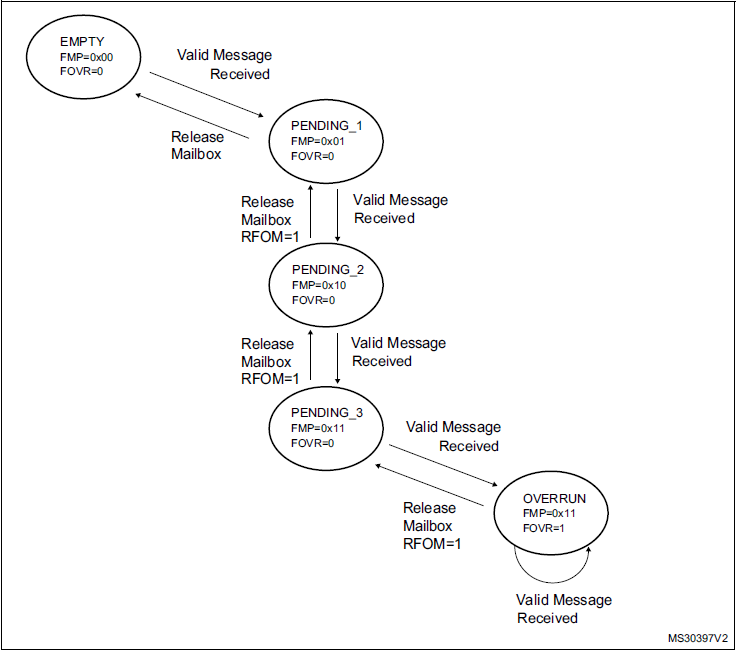
\includegraphics[width=\textwidth]{receive_fifo_states.png}
	\caption{Stanja prijemnih FIFO strukuta \cite{l471_manual}}
	\label{fig:receive_fifo_states}
\end{figure}
Upravljanje FIFO strukturom ilustrirano je slikom \ref{fig:receive_fifo_states}. Počevši od praznog stanja \engl{empty}, prva primljena ispravna poruka se sprema u FIFO strukturu koja prelazi u \textit{pending\_1} stanje. Sklopovlje signalizira taj događaj postavljanjem bitova FMP[1:0] u CAN\_RFR registru na vrijednost 01b. Poruka postaje dostupna u izlaznoj FIFO \textit{mailbox} strukturi. Programska podrška pročita sadržaj \textit{mailbox} te ju otpušta postavljanjem RFOM bita u CAN\_RFR registru, te FIFO struktura ponovno postane prazna. Ako je, u međuvremenu, primljena još jedna ispravna poruka FIFO struktura ostaje u \textit{pending\_1} stanju i nova poruka je dostupna u izlaznoj FIFO \textit{mailbox} strukturi. Ako aplikacija ne otpusti \textit{mailbox} strukturu, sljedeća ispravna poruka se sprema u FIFO strukturu te se ulazi u \textit{pending\_2} stanje(FMP[1:0]=10b). Proces pohrane se ponavlja za sljedeću ispravnu poruku te FIFO ulazi u \textit{pending\_3} stanje (FMP[1:0]=11b). U ovom trenutku programska podrška mora otpustiti \textit{mailbox} strukturu postavljanjem RFOM bita, kako bi struktura bila dostupna za pohranu sljedeće ispravne poruke, u suprotnom sljedeća ispravna poruka uzrokuje gubitak poruke.

Kada je FIFO struktura u \textit{pending\_3} stanju, sljedeća ispravna poruka dovodi do prekoračenja i poruka se gubi. Sklopovlje signalizira prekoračenje postavljanjem FOVR bita u CAN\_RFR registru. Koja se poruka točno gubi ovisi o konfiguraciji FIFO strukture:
\begin{itemize}
	\item ako je funkcija zaključivanja FIFO strukture isključena (RFLM bit u CAN\_MCR registru je očišćen) posljednja poruka koja je pohranjena u FIFO strukturi se prepisuje novom porukom. U ovom slučaju najnovija poruka je uvijek dostupna aplikaciji,
	\item ako je funkcija zaključivanja FIFO strukture uključena (RFLM bit u CAN\_MCR registru je postavljen u jedinicu) najnovija poruka se odbacuje i programska podrška ima pristup trima najstarijim porukama.
\end{itemize}

Jednom kada se poruka pohrani u FIFO strukturu, ažuriraju se bitovi FMP[1:0] i generira se zahtjev za prekidom, pod uvijetom da je FMPIE bit u CAN\_IER registru postavljen u visoku logičku razinu. Kada FIFO struktura postane puna FULL bit u CAN\_RFR registru se postavlja u visoku logičku razinu i generira se zahtjev za prekid, pod uvijetom da je FFIE bit u CAN\_IER registru postavljen u jedinicu. Ako je FOVR bit u CAN\_IER registru postavljen u jedinicu, generira se zahtijev za prekidom svaki put kada se dogodi prekoračenje.

\paragraph{Filtriranje identifikatora}

U CAN protokolu identifikator poruke nije povezan s adresom čvora nego je povezan sa sadržajem poruke. Posljedično, odašiljač šalje svoju poruku svim čvorovima. Na primitak poruke čvor odlučuje da li mu je poruka potrebna ili ne, ovisno o vrijednosti identifikatora. Ako je poruka potrebna kopira se u SRAM, a ako nije onda se odbacuje bez intervencije programske podrške. Kako bi se ispunio ovaj zahtjev, na raspolaganju su 14 podesivih i skalabilnih banaka filtera. Svaka banka filtera se sastoji od da 32-bitna registra, CAN\_FxR0 i CAN\_FxR1.

Kako bi se filteri optimizirali i prilagodili prema potrebama aplikacije, svaka banka filtera se može neovisno skalirati. Ovisno o skali filtera, banka filtera pruža:
\begin{itemize}
	\item jedan 32-bitni filter za STDIT[10:0], EXTID[17:0], IDE i RTR bitove,
	\item dva 16-bitna filtra za STDIT[10:0], RTR, IDE i EXTID[17:15].
\end{itemize}
\noindent Filteri mogu biti podešeni tako da rade u maskiranom načinu rada ili u načinu rada s popisom identifikatora. U maskiranom načinu rada identifikatorski registri su povezani s registrima maske koja određuje koji bitovi identifikatora se moraju podudarati \engl{must match} ili koji nisu bitni \engl{don't care}. U načinu rada s popisom identifikatora registri maske se koriste kao identifikatorski registri. Tako umjesto da se definira identifikator i maska, definiraju se dva identifikatora. Svi se bitovi nadolazećeg identifikatora moraju podudarati s bitovima specificiranim u registrima filtra.

Banke filtera se podešavaju preko odgovarajućeg CAN\_FMR registra. Kako bi se podesila banka filtera, prvo se mora deaktivirati banka čišćenjem FACT bita u CAN\_FAR registru. Skala filtera se podešava preko odgovarajućeg FSCx bita u CAN\_FS1R registru. Način rada za odgovarajuće registre maske ili identifikatorske registre se podešava preko FBMx bita u CAN\_FMR registru.

Jednom kada FIFO struktura primi poruku, ona je dostupna aplikaciji. Aplikacijski podaci se obično kopiraju u neku lokaciju u SRAM memoriji. Kako bi se podatak kopirao na pravu lokaciju, aplikacija mora identificirati podatak uz pomoć identifikatora. Kako bi se to izbjeglo i olakšalo pristup lokacijama u SRAM memoriji, CAN kontroler pruža indeks podudaranja filtra. Indeks se pohranjuje u \textit{mailbox} strukturu zajedno sa porukom prema pravilima prioriteta filtra. Tako svaka primljena poruka ima pridružen indeks podudaranja filtra. Index podudaranja filtra se može iskoristiti na dva načina:
\begin{itemize}
	\item uspoređivanje indeksa s popisom očekivanih vrijednosti,
	\item korištenje indeksa na nizu za pristup lokaciji podatka.
\end{itemize}
Za nemaskirane filtre programska podrška ne treba uspoređivati identifikator. Ako je filter maskiran programska podrška smanjuje uspoređivanje samo na maskirane bitove.

Pravila prioriteta filtra.

Ovisno o kombinaciji filtra može se dogoditi da identifikator prođe uspješno kroz nekoliko filtera. U ovom slučaju vrijednost podudaranja filtra pohranjena u primajućoj \textit{mailbox} strukturi se odabire prema sljedećim pravilima prioriteta:
\begin{itemize}
	\item 32-bitni filtar ima veći prioritet od 16-bitnog filtra,
	\item za filtre jednake skale, prioritet se daje filtru s načinom rada s popisom identifikatora, a ne filtru s maskiranim načinom rada,
	\item za filtre s istom skalom i načinom rada, prioritet se određuje prema broju filtra (manji broj, veći prioritet).
\end{itemize}

\paragraph{Pohrana poruke}

Sučelje između programske podrške i sklopovlja za CAN poruke je implementirano preko \textit{mailbox} struktura. \textit{Mailbox} struktura sadržava sve informacije povezane s porukom; informacije o identifikatoru, podacima, kontroli, statusu i vremenskoj oznaci.

Programska podrška sastavlja poruku koja se treba poslati u praznoj \textit{mailbox} strukturi. Status odašiljanja naznačuje sklopovlje u CAN\_TSR registru.

Kada se poruka primi, ona je dostupna programskoj podršci u FIFO izlaznoj \textit{mailbox} strukturi. Kada programska podrška pročita poruku, programska podrška mora otpustiti \textit{mailbox} strukturu preko RFOM bita u CAN\_RFR registru kako bi sljedeća nadolazeća poruka bila dostupna. Indeks podudaranja filtera se pohranjuje u MFMI polju u CAN\_RDTxR registru. 16-bitna vrijednost vremenske oznake se pohranjuje u TIME[15:0] polju u CAN\_RDTxR registru.

\paragraph{Upravljanje pogreškama}

Upravljanje pogreškama kao što je opisano u CAN protokolu odrađuje sklopovlje koristeći brojač odašiljačkih pogrešaka (engl. \textit{Transmit Error Counter}, TEC vrijednost u CAN\_ESR registru) i brojač prijamničkih pogrešaka (engl. Receive Error Counter, REC vrijednost u CAN\_ESR registru) koji se inkrementiraju ili dekrementiraju ovisno o stanju pogreške. Obje vrijednosti se mogu pročitati kako bi se ustanovila stabilnost mreže. Nadalje, CAN sklopovlje pruža detaljne informacije o trenutačnom statusu greške u CAN\_ESR registru. Preko CAN\_IER registra programska podrška može podesiti stvaranje prekida na detekciju pogreške.

Kada je vrijednost TEC polja veća od 255 dolazi do \textit{Bus-Off} stanja koje je naznačeno preko BOFF bita u CAN\_ESR polju. U \textit{Bus-Off} stanju bxCAN periferija više ne može slati i primati poruke. Ovisno o ABOM bitu u CAN\_MCR registru, bxCAN se oporavi od \textit{Bus-Off} stanja automatski ili na zahtjev programske podrške. U oba slučaja bxCAN mora čekati redoslijed oporavka specificiran u CAN standardu (128 pojava 11 uzastopnih recesivnih bitova na CANRX liniji).

\paragraph{Vrijeme bita}

Logika vremena bita nadzire liniju serijske sabirnice i izvodi uzorkovanje i podešavanje točke uzorkovanja sinkronizacijom na rubu početnog bita i ponovnom sinkronizacijom na sljedećem rubovima.

Način rada logike vremena bita se može objasniti dijeljenjem nominalnog vremena bita na tri segmenta (slika \ref{fig:bit_timing}):
\begin{itemize}
	\item sinkronizacijski segment (SYNC\_SEG) - u ovom segmentu se očekuje promjena bita. Njegova duljina je fiksna i iznosi jedan vremenski kvant (1 x t\textsubscript{q}),
	\item prvi segment bita (BS1) - određuje lokaciju točke uzorkovanja. Njegovo trajanje je programabilno između 1 i 16 vremenskih kvanta, ali može se automatski produžiti kako bi se kompenzirao pozitivni fazni pomak koji nastaje radi razlika u frekvencijama raznih čvorova na mreži,
	\item drugi segment bita (BS2) - određuje lokaciju točke odašiljanja. Njegovo trajanje je programabilno između 1 i 8 vremenskih kvanti, ali može se automatski smanjiti kako bi se kompenzirao negativni fazni pomak.
\end{itemize}

Širina skoka ponovne sinkronizacije (\textit{resynchronization jump width}, SJW) određuje gornju granicu iznosa produženja ili skraćivanja segmenata bita. Programabilna je između 1 i 4 vremenskih kvanta.

Valjan rub se definira kao prva promjena u vremenu bita iz dominantnog u recesivno stanje sabirnice, pod uvjetom da kontroler sam ne pošalje recesivni bit. Ako se valjani rub detektira u BS1 umjesto SYNC\_SEG, BS1 se produžuje za do SJW, kako bi se odgodila točka uzorkovanja. Ako se valjanu rub detektira u BS2 umjesto u SYNC\_SEG, BS2 se skraćuje za do SJW, kako bi se točka odašiljanja pomaknula ranije.

\begin{figure}[H]
	\centering
	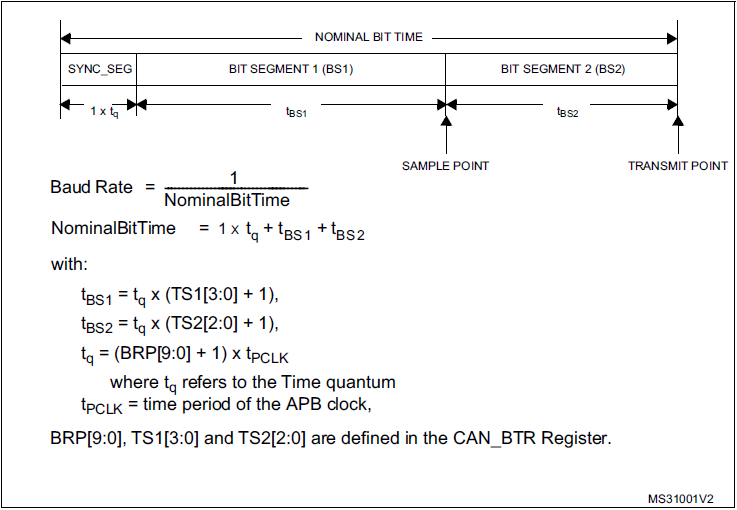
\includegraphics[width=\textwidth]{bit_timing.png}
	\caption{Prikaz i proračun vremena bita \cite[str. 1645]{l471_manual}}
	\label{fig:bit_timing}
\end{figure}

\begin{table}[H]
	\caption{Registri CAN periferije kod STM32L471VGT6 mikrokontrolera \citep[poglavlje 46]{l471_manual}}
	\resizebox{\textwidth}{!}{%
	\begin{tabular}{|c|c|l|l|l|l|l|l|l|l|l|l|l|l|l|l|l|l|l|l|l|l|l|l|l|l|l|l|l|l|l|l|l|}
		\hline
		\textbf{\begin{tabular}[c]{@{}c@{}}Register\\ name\end{tabular}} & \rotbf{31} & \rotbf{30} & \rotbf{29} & \rotbf{28} & \rotbf{27} & \rotbf{26} & \rotbf{25} & \rotbf{24} & \rotbf{23} & \rotbf{22} & \rotbf{21} & \rotbf{20} & \rotbf{19} & \rotbf{18} & \rotbf{17} & \rotbf{16} & \rotbf{15} & \rotbf{14} & \rotbf{13} & \rotbf{12} & \rotbf{11} & \rotbf{10} & \rotbf{9} & \rotbf{8} & \rotbf{7} & \rotbf{6} & \rotbf{5} & \rotbf{4} & \rotbf{3} & \rotbf{2} & \rotbf{1} & \rotbf{0} \\
		\hline
		CAN\_MCR & \multicolumn{15}{c|}{Res.} & \rot{DBF} & \rot{RESET} & \multicolumn{7}{c|}{Res.} & \rot{TTCM} & \rot{ABOM} & \rot{AWUM} & \rot{NART} & \rot{RFLM} & \rot{TXFP} & \rot{SLEEP} & \rot{INRQ} \\
		\hline
		Reset value & & & & & & & & & & & & & & & & 1 & 0 & & & & & & & & 0 & 0 & 0 & 0 & 0 & 0 & 1 & 0 \\
		\hline
		CAN\_MSR & \multicolumn{20}{c|}{Res.} & \rot{RX} & \rot{SAMP} & \rot{RXM} & \rot{TXM} & \multicolumn{3}{c|}{Res.} & \rot{SLAKI} & \rot{WKUI} & \rot{ERRI} & \rot{SLAK} & \rot{INAK} \\
		\hline
		Reset value & & & & & & & & & & & & & & & & & & & & & 1 & 1 & 0 & 0 & & & & 0 & 0 & 0 & 1 & 0 \\
		\hline
		CAN\_TSR & \multicolumn{3}{c|}{\rot{LOW[2:0]}} & \multicolumn{3}{c|}{\rot{TME[2:0]}} & \multicolumn{2}{c|}{\rot{CODE[1:0]}} & \rot{ABRQ2} & \multicolumn{3}{c|}{Res.} & \rot{TERR2} & \rot{ALST2} & \rot{TXOK2} & \rot{RQCP2} & \rot{ABRQ1} & \multicolumn{3}{c|}{Res.} & \rot{TERR1} & \rot{ALST1} & \rot{TXOK1} & \rot{RQCP1} & \rot{ABRQ0} & \multicolumn{3}{c|}{Res.} & \rot{TERR0} & \rot{ALST0} & \rot{TXOK0} & \rot{RQCP0} \\
		\hline
		Reset value & 0 & 0 & 0 & 1 & 1 & 1 & 0 & 0 & 0 & & & & 0 & 0 & 0 & 0 & 0 & & & & 0 & 0 & 0 & 0 & 0 & & & & 0 & 0 & 0 & 0 \\
		\hline
		CAN\_RF0R & \multicolumn{26}{c|}{Res.} & \rot{RFOM0} & \rot{FOVR0} & \rot{FULL0} & \rot{Res.} & \multicolumn{2}{c|}{\rot{FMP0[1:0]}} \\
		\hline
		Reset value & & & & & & & & & & & & & & & & & & & & & & & & & & & 0 & 0 & 0 & & 0 & 0 \\
		\hline
		CAN\_RF1R & \multicolumn{26}{c|}{Res.} & \rot{RFOM1} & \rot{FOVR1} & \rot{FULL1} & \rot{Res.} & \multicolumn{2}{c|}{\rot{FMP1[1:0]}} \\
		\hline
		Reset value & & & & & & & & & & & & & & & & & & & & & & & & & & & 0 & 0 & 0 & & 0 & 0 \\
		\hline
		CAN\_IER & \multicolumn{14}{c|}{Res.} & \rot{SLKIE} & \rot{WKUIE} & \rot{ERRIE} & \multicolumn{3}{c|}{Res.} & \rot{LECIE} & \rot{BOFIE} & \rot{EPVIE} & \rot{EWGIE} & \rot{Res.} & \rot{FOVIE1} & \rot{FFIE1} & \rot{FMPIE1} & \rot{FOVIE0} & \rot{FFIE0} & \rot{FMPIE0} & \rot{TMEIE} \\
		\hline
		Reset value & & & & & & & & & & & & & & & 0 & 0 & 0 & & & & 0 & 0 & 0 & 0 & & 0 & 0 & 0 & 0 & 0 & 0 & 0 \\
		\hline
		CAN\_ESR & \multicolumn{8}{c|}{REC[7:0]} & \multicolumn{8}{c|}{TEC[7:0]} & \multicolumn{9}{c|}{Res.} & \multicolumn{3}{c|}{\rot{LEC[2:0]}} & \rot{Res.} & \rot{BOFF} & \rot{EPVF} & \rot{EWGF} \\
		\hline
		Reset value & 0 & 0 & 0 & 0 & 0 & 0 & 0 & 0 & 0 & 0 & 0 & 0 & 0 & 0 & 0 & 0 & & & & & & & & & & 0 & 0 & 0 & & 0 & 0 & 0 \\
		\hline
		CAN\_BTR & \rot{SILM} & \rot{LBKM} & \multicolumn{4}{c|}{Rot.} & \multicolumn{2}{c|}{\rot{SJW[1:0]}} & \rot{Res.} & \multicolumn{3}{c|}{TS2[2:0]} & \multicolumn{4}{c|}{TS1[3:0]} & \multicolumn{6}{c|}{Res} & \multicolumn{10}{c|}{BRP[9:0]} \\
		\hline
		Reset value & 0 & 0 & & & & & 0 & 0 & & 0 & 1 & 0 & 0 & 0 & 1 & 1 & & & & & & & 0 & 0 & 0 & 0 & 0 & 0 & 0 & 0 & 0 & 0 \\
		\hline
		CAN\_TIxR & \multicolumn{11}{c|}{STID[10:0]/EXID[28:18]} & \multicolumn{18}{c|}{EXID[17:0]} & \rot{IDE} & \rot{RTR} & \rot{TXRQ} \\
		\hline
		Reset value & X & X & X & X & X & X & X & X & X & X & X & X & X & X & X & X & X & X & X & X & X & X & X & X & X & X & X & X & X & X & X & 0 \\
		\hline
		CAN\_TDTxR & \multicolumn{16}{c|}{TIME[15:0]} & \multicolumn{7}{c|}{Res.} & \rot{TGT} & \multicolumn{4}{c|}{Res.} & \multicolumn{4}{c|}{DLC[3:0]} \\
		\hline
		Reset value & X & X & X & X & X & X & X & X & X & X & X & X & X & X & X & X & & & & & & & & X & & & & & X & X & X & X \\
		\hline
		CAN\_TDLxR & \multicolumn{8}{c|}{DATA3[7:0]} & \multicolumn{8}{c|}{DATA2[7:0]} & \multicolumn{8}{c|}{DATA1[7:0]} & \multicolumn{8}{c|}{DATA0[7:0]} \\
		\hline
		Reset value & X & X & X & X & X & X & X & X & X & X & X & X & X & X & X & X & X & X & X & X & X & X & X & X & X & X & X & X & X & X & X & X \\
		\hline
		CAN\_TDHxR & \multicolumn{8}{c|}{DATA7[7:0]} & \multicolumn{8}{c|}{DATA6[7:0]} & \multicolumn{8}{c|}{DATA5[7:0]} & \multicolumn{8}{c|}{DATA4[7:0]} \\
		\hline
		Reset value & X & X & X & X & X & X & X & X & X & X & X & X & X & X & X & X & X & X & X & X & X & X & X & X & X & X & X & X & X & X & X & X \\
		\hline
		CAN\_RIxR & \multicolumn{11}{c|}{STID[10:0]/EXID[28:18]} & \multicolumn{18}{c|}{EXID[17:0]} & \rot{IDE} & \rot{RTR} & \rot{Res.} \\
		\hline
		Reset value & X & X & X & X & X & X & X & X & X & X & X & X & X & X & X & X & X & X & X & X & X & X & X & X & X & X & X & X & X & X & X & X \\
		\hline
		CAN\_RDTxR & \multicolumn{16}{c|}{TIME[15:0]} & \multicolumn{8}{c|}{FMI[7:0]} & \multicolumn{4}{c|}{Res.} & \multicolumn{4}{c|}{DLC[3:0]} \\
		\hline
		Reset value & X & X & X & X & X & X & X & X & X & X & X & X & X & X & X & X & X & X & X & X & X & X & X & X & X & X & X & X & X & X & X & X \\
		\hline
		CAN\_RDLxR & \multicolumn{8}{c|}{DATA3[7:0]} & \multicolumn{8}{c|}{DATA2[7:0]} & \multicolumn{8}{c|}{DATA1[7:0]} & \multicolumn{8}{c|}{DATA0[7:0]} \\
		\hline
		Reset value & X & X & X & X & X & X & X & X & X & X & X & X & X & X & X & X & X & X & X & X & X & X & X & X & X & X & X & X & X & X & X & X \\
		\hline
		CAN\_RDHxR & \multicolumn{8}{c|}{DATA7[7:0]} & \multicolumn{8}{c|}{DATA6[7:0]} & \multicolumn{8}{c|}{DATA5[7:0]} & \multicolumn{8}{c|}{DATA4[7:0]} \\
		\hline
		Reset value & X & X & X & X & X & X & X & X & X & X & X & X & X & X & X & X & X & X & X & X & X & X & X & X & X & X & X & X & X & X & X & X \\
		\hline
		CAN\_FMR & \multicolumn{18}{c|}{Res.} & \multicolumn{6}{c|}{CANSB[5:0]} & \multicolumn{7}{c|}{Res.} & \rot{FINIT} \\
		\hline
		Reset value & & & & & & & & & & & & & & & & & & & 0 & 0 & 1 & 1 & 1 & 0 & & & & & & & & 1 \\
		\hline
		CAN\_FM1R & \multicolumn{4}{c|}{Res.} & \multicolumn{28}{c|}{FMB[27:0]} \\
		\hline
		Reset value & & & & & 0 & 0 & 0 & 0 & 0 & 0 & 0 & 0 & 0 & 0 & 0 & 0 & 0 & 0 & 0 & 0 & 0 & 0 & 0 & 0 & 0 & 0 & 0 & 0 & 0 & 0 & 0 & 0 \\
		\hline
		CAN\_FS1R & \multicolumn{4}{c|}{Res.} & \multicolumn{28}{c|}{FSC[27:0]} \\
		\hline
		Reset value & & & & & 0 & 0 & 0 & 0 & 0 & 0 & 0 & 0 & 0 & 0 & 0 & 0 & 0 & 0 & 0 & 0 & 0 & 0 & 0 & 0 & 0 & 0 & 0 & 0 & 0 & 0 & 0 & 0 \\
		\hline
		CAN\_FFA1R & \multicolumn{4}{c|}{Res.} & \multicolumn{28}{c|}{FFA[27:0]} \\
		\hline
		Reset value & & & & & 0 & 0 & 0 & 0 & 0 & 0 & 0 & 0 & 0 & 0 & 0 & 0 & 0 & 0 & 0 & 0 & 0 & 0 & 0 & 0 & 0 & 0 & 0 & 0 & 0 & 0 & 0 & 0 \\
		\hline
		CAN\_FA1R & \multicolumn{4}{c|}{Res.} & \multicolumn{28}{c|}{FACT[27:0]} \\
		\hline
		Reset value & & & & & 0 & 0 & 0 & 0 & 0 & 0 & 0 & 0 & 0 & 0 & 0 & 0 & 0 & 0 & 0 & 0 & 0 & 0 & 0 & 0 & 0 & 0 & 0 & 0 & 0 & 0 & 0 & 0 \\
		\hline
		CAN\_FiRx & \multicolumn{32}{c|}{FB[31:0]} \\
		\hline
		Reset value & X & X & X & X & X & X & X & X & X & X & X & X & X & X & X & X & X & X & X & X & X & X & X & X & X & X & X & X & X & X & X & X \\
		\hline
	\end{tabular}%
	}
	\label{Tab:f407_dma_register_map_2}
\end{table}
\chapter{Programska podrška}

Prilikom razvoja programske podrške korišteno je integrirano razvojno okruženje STM32CubeIDE, PDH sustav i programator ST-LINK/V2. Programska potpora razvijena je u jeziku C uz korištenje GCC prevodioca.

\section{Korišteni programski paketi i biblioteke}

Razvojno okruženje STM32CubeIDE nudi mogućnost grafičkog podešavanja parametara periferija i automatsko generiranje koda, čime su olakšane inicijalizacije raznih perifernih sklopova. Prije generiranja koda moguće je odabrati hoće li se koristiti HAL \engl(Hardware Abstraction Layer) ili LL \engl{Low-Layer} biblioteke.

HAL biblioteke nude visoku razinu abstrakcije i lakše su za koristiti, međutim, one rade po principu "crne kutije", te ih stoga korisnik teže razumije. HAL funkcije također zauzimaju više radne memorije od LL funkcije jer u sebi sadržavaju kojekakve provjere vrijednosti i modifikacije unutarnjih HAL struktura, pa time nisu osigurane optimalne performanse.

Iz tog razloga odlučeno je da će se koristiti LL biblioteke. LL funkcije omogućuju izravan pristup registrima periferija i korisnik ih daleko jednostavnije razumije, s obzirom na to da se često sastoje od samo jedne linije koda.

\section{Programska potpora za kameru}

Za rad s kamerom razvijene su korisničke funkcije prikazane u isječku \ref{lst:arducam_code}.

\begin{lstlisting}[caption=Korisničke funkcije za Arducam 5MP Mini Plus, label={lst:arducam_code}]
uint8_t ACAM_TestComms(void);
uint8_t ACAM_SPI_Read(uint8_t reg);
void ACAM_SPI_Write(uint8_t reg, uint8_t val);
void ACAM_spi_read_package(uint8_t * buff, uint16_t size);
void ACAM_I2C_Setup();
uint8_t ACAM_I2C_Read(uint16_t reg);
void ACAM_I2C_Write(uint16_t reg, uint8_t command);
void ACAM_I2C_WriteSeq(const struct ACAM_I2C_Register commandSeq[]);
uint8_t ACAM_TestComms(void);
void ACAM_select_JPEG(void);
void ACAM_select_RAW(uint8_t resolution);
void ACAM_start_capture(void);
uint32_t ACAM_get_image_size();
void ACAM_set_exposure(uint16_t nr_lines, uint8_t nr_lines_frac);
void ACAM_Reset(void);
void ACAM_exp_gain_manual(void)
void ACAM_exp_gain_auto(void)
uint8_t ACAM_is_cap_complete(void)
void ACAM_set_gain(uint8_t gain);
\end{lstlisting}

Za testiranje SPI i I\textsuperscript{2}C komunikacija između mikrokontrolera i kamere postoji funkcija \verb|ACAM_TestComms()|, za odabir između RAW i JPEG formata slike na raspolaganju su funkcije \verb|ACAM_select_RAW()| i \verb|ACAM_select_JPEG()|. Način upravljanja ekspozicijom odabire se funkcijama \verb|ACAM_exp_gain_manual()| i \verb|ACAM_exp_gain_auto()|, a ukoliko se odabere ručni način upravljanja ekspozicijom parametri vremena ekspozicije i pojačanja pojačala se podešavaju funkcijama \verb|ACAM_set_exposure()| i \verb|ACAM_set_gain()|. Komanda za početak slikanja se šalje funkcijom \verb|ACAM_start_capture()|, a provjera završetka slikanja se obavlja funkcijom \verb|ACAM_is_cap_complete()|. Navedene funkcije nije trebalo mijenjati u odnosu na prethodnu programsku podršku, pa one rade na isti način kao i u prethodnom radu \cite{diplomski_goran_petrak}. Funkcije koje direktno rade sa SPI i I\textsuperscript{2}C periferijom su jedine mijenjane s obzirom na to da se rad periferija između prethodno korištenog i trenutačno korištenog mikrokontrolera razlikuju, kako je i pokazano u poglavlju 3. U nastavku će biti istaknute razlike između starih i novih funkcija kao i obrazloženje radi čega je došlo do promjena.

\subsection{Funkcije za rad sa I\textsuperscript{2}C periferijom}

Funkcije za rad s I\textsuperscript{2}C periferijom navedene su u isječku \ref{lst:acam_i2c_functions}.

\begin{lstlisting}[caption=Funkcije za rad s I\textsuperscript{2}C periferijom, label={lst:acam_i2c_functions}]
void ACAM_I2C_Setup();
uint8_t ACAM_I2C_Read(uint16_t reg);
void ACAM_I2C_Write(uint16_t reg, uint8_t command);
void ACAM_I2C_WriteSeq(const struct ACAM_I2C_Register commandSeq[]);
\end{lstlisting}

U odnosu na prethodnu programsku podršku dodana je funkcija \verb|ACAM_I2C_Setup()| koja podešava I\textsuperscript{2}C periferiju. Funkcija postavlja adresu uređaja s kojim se želi komunicirati, odnosno SADD registar, i govori periferiji želi li se na uređaj nešto čitati ili pisati, odnosno podešava RD\_WRN bit u I2C\_CR2 registru. Tu funkciju je važno pozvati prije svakog pokušaja komunikacije s kamerom. Funkcije \verb|ACAM_I2C_Write()|,  \verb|ACAM_I2C_Read()| i \verb|ACAM_I2C_WriteSeq()| služe za prijenos podataka između kamere i mikrokontrolera, i one su prošle manje promjene, konkretno, bilo je potrebno omogućiti drugačije prekide i provjeravati drugačije statusne zastavice, zato što registarska mapa I\textsuperscript{2}C periferije izgleda drugačije na STM32L471VGT6 mikrokontroleru nego na STM32F407VGT6 mikrokontroleru. Navedene promjene nije bilo teško implementirati zato što LL funkcije koriste intuitivna imena. Na primjer, funkcija koja omogućava TC prekid (prekid za završetak prijenosa) je \verb|LL_I2C_EnableIT_TC()|, a funkcija koja provjerava da li je podignuta zastavica BUSY (prijenos je u tijeku) je \verb|LL_I2C_IsActiveFlag_Busy()|.

Prijenos preko I\textsuperscript{2}C protokola u ovom radu funkcionira tako da se u jednoj od funkcija koje su zadužene za prijenos podataka postavi adresa uređaja s kojim se želi komunicirati (u ovom slučaju kamera), nakon toga generira se \textit{start} uvjet i omogućuju se prekidi relevantni za vrstu prijenosa koja se želi obaviti (slanje ili primanje podataka). Stanje komunikacije se prati preko globalne zastavice koja se osvježava u prekidnoj podrutini \verb|I2C1_EV_IRQHandler()|. Jedina promjena koju je prekidan funkcija doživjela jest ta da je izbrisan kod za provjeru je li poslana adresa \textit{slave} uređaja. Naime, na prethodno korištenom mikrokontroleru nije postojao posebni registar za adresu \textit{slave} uređaja, nego se adresa slala preko izlaznog registra periferiju. Kod novog mikrokontrolera, čim se pošalje \textit{start} bit šalje se adresa \textit{slave} uređaja preko SADD registra i automatski se provjerava da ACK bit za potvrdu primitka točne adrese \textit{slave} uređaja. Ostatak funkcije funkcionira na isti način kao i na prethodnom mikrokontroleru.

\subsection{Funkcije za rad sa SPI periferijom}

Funkcije za rad s SPI periferijom navedene su u isječku \ref{lst:acam_spi_functions}.

\begin{lstlisting}[caption=Funkcije za rad s SPI periferijom, label={lst:acam_spi_functions}]
uint8_t ACAM_SPI_Read(uint8_t reg);
void ACAM_SPI_Write(uint8_t reg, uint8_t val);
void ACAM_spi_read_package(uint8_t * buff, uint16_t size);
\end{lstlisting}

\section{Učitavanje programa}

Kako bi se programska podrška mogla učitati na mikrokontroler PDH sustava nužno je koristiti programator, u ovom slučaju ST-LINK/V2. Na raspolaganju je STM32F4DISCOVERY razvojni sustav koji ima ugrađen ST-LINK/V2 programator. Programator na razvojnom sustavu se može koristiti za programiranje mikrokontrolera na razvojnom sustavu ili programiranje mikrokontrolera na vanjskoj pločici. Koji mikrokontroler programator programira određuju prespojnici CN3 na razvojnom sustavu:
\begin{itemize}
	\item ako su oba prespojnika spojena, programira se mikrokontroler na razvojnom sustavu,
	\item ako su oba prespojnika odspojena, programira se mikrokontroler na vanjskoj pločici.
\end{itemize}
Programiranje se izvodi preko CN2 konektora na razvojnom sustavu i X6 konektora na PDH sustavu. Funkcije stezaljki na pojedinim konektorima su dane u tablici \ref{Tab:conn_func}.
\begin{center}
	\begin{table}[H]
		\centering
		\caption{Opis stezaljki CN2 i X6 konektora \cite{zavrsni_filip_juric}, \cite{disc_manual}}
		\begin{tabular}{| c | c | c |}
			\hline
			Redni broj stezaljke & CN2 & X6 \\
			\hline
			1. & VDD & VDD \\
			\hline
			2. & SWCLK & SWDIO \\
			\hline
			3. & GND & SWCLK \\
			\hline
			4. & SWDIO & SWO \\
			\hline
			5. & NRST & NRST \\
			\hline
			6. & SWO & GND \\
			\hline
		\end{tabular}
		\label{Tab:conn_func}
	\end{table}
\end{center}
Potrebno je spojiti istoimene stezaljke kako bi se učitavanje programa uspješno izvelo. Osim za programiranje, razvojni sustav se koristi kako bi PDH sustav imao napajanje, s obzirom na to da sustav napajanja na PDH sustavu trenutačno nije ispravno.
\chapter{Rezultati}

S obzirom da CDH računalo nije dostupno u trenutku pisanja ovog rada,
komunikacija PDH računala s CDH računalom emulira se kroz komunikaciju s osobnim računalom
putem sučelja USART.
Na osobnom računalu potrebno je koristiti emulator terminala koji može koristiti UART komunikaciju. U tu svrhu odabran je program CoolTerm, 
koji može primati i slati podatke preko UART sučelja i može spremati  
primljene podatke, što je potrebno kako bi se na računalu mogla učitati slika s kamere. 
Brzina prijenosa putem UART sučelja postavljena je na 115200 bit/s.
Za obradu naredbi primljenih s osobnog računala korištena 
je programska potpora razvijena u okviru prethodnog rada \cite{diplomski_goran_petrak}.

Kada se sustav uključi prvo se ispisuje rezultat inicijalizacije sustava. Ako je inicijalizacija uspješna, ispisuje se poruka \verb|startup_ok|. Nakon toga nudi se izbor ponovne inicijalizacije datotečnog sustava, te se nudi izbor datoteke za slanje. Ako korisnik želi, može odmah nakon slanja datoteke odabranu datoteku izbrisati, a može i izbrisati datoteke bez prethodnog slanja. Korisnik može odabrati da se slanje datoteka preskoči. Sustav zatim traži od korisnika da koristi uobičajene, odnosne prethodne, postavke kamere ili da sam podesi postavke kamere ili da se korištenje kamere preskoči. Ako korisnik odabere da želi podesiti postavke kamere, sustav mu nudi da podesi vrijeme ekspozicije (\verb|nr_lines| za cjelobrojni dio i \verb|nr_lines_frac| za frakcionalni dio trajanja vremena ekspozicije), pojačanje pojačala (\verb|gain|) i format spremanja slike. Kada korisnik konfigurira postavke sustava i odabere željene funkcionalnosti,
sustav ponudi korisniku pokretanje operacija PDH sustava. Kada sustav završi s izvršavanjem operacija ispisuje se rezultat operacija i status sustava, te sustav krene ispočetka i ponovno ponudi korisniku reinicijalizaciju datotečnog sustava. Primjer komunikacije između računala i PDH sustava dan je u isječku koda \ref{lst:default_comms}.

\begin{lstlisting}[caption=Komunikacija između računala i PDH sustava, label={lst:default_comms}]
sustav: startup_ok
sustav: Type 'reinit' to reinitialize the filesystem, 'n' not to
korisnik: n
sustav: Press 'y' to select file for transmission, 'n' to skip
korisnik: n
sustav: Any [other] file you would like to delete?['y'/'n']
korisnik: n
sustav: Press 'y' to set camera params, 'd' to use default/previous, 'n' to skip
korisnik: y
sustav: Set exposure nr_lines (uint16_t).
korisnik: 2000
sustav: Set exposure nr_lines frac (uint8_t).
korisnik: 10
sustav: Set gain (uint8_t), see acam.h.
korisnik: 9
sustav: Select format: 'r' for raw, 'j' for jpeg,
korisnik: j
sustav: Enter file name [0-1023] to store image measurments.
korisnik: 0
sustav: Press 's' to start PDH operations
korisni: s
sustav: Device camera status ok
sustav: Type 'reinit' to reinitialize the filesystem, 'n' not to
korisnik: n
sustav: Press 'y' to select file for transmission, 'n' to skip
korisnik: y
sustav: Enter file name [0-1023] of file to be transmitted via x-band.
korisnik: 0
sustav: Press 'y' to delete file after transmission, 'n' to keep it
korisnik: y
sustav: Any [other] file you would like to delete?['y'/'n']
korisnik: n
sustav: Press 'y' to set camera params, 'd' to use default/previous, 'n' to skip
korisnik: n
sustav: Press 's' to start PDH operations
korisnik: s
sustav: ÿØÿ
...
slanje slike
...
ÿÙ Device xband status ok
sustav: Type 'reinit' to reinitialize the filesystem, 'n' not to
\end{lstlisting}

Ovisno o svjetlini okoline gdje se nalazi kamera preporučuje se vrijednost cjelobrojnog dijela vremena ekspozicije 2000 za relativno svjetlo područje i 5000 za relativno mračno područje. Za frakcionalni dio vremena ekspozicije preporučuje se mala vrijednost, na primjer 10. Isto tako, male vrijednosti se preporučuju za pojačanje pojačala. Primjer slika koje su uslikane s navedenim parametrima u \textit{jpeg} formatu prikazane su na slikama \ref{fig:dark} i \ref{fig:light}.
\begin{figure}[H]
	\centering
	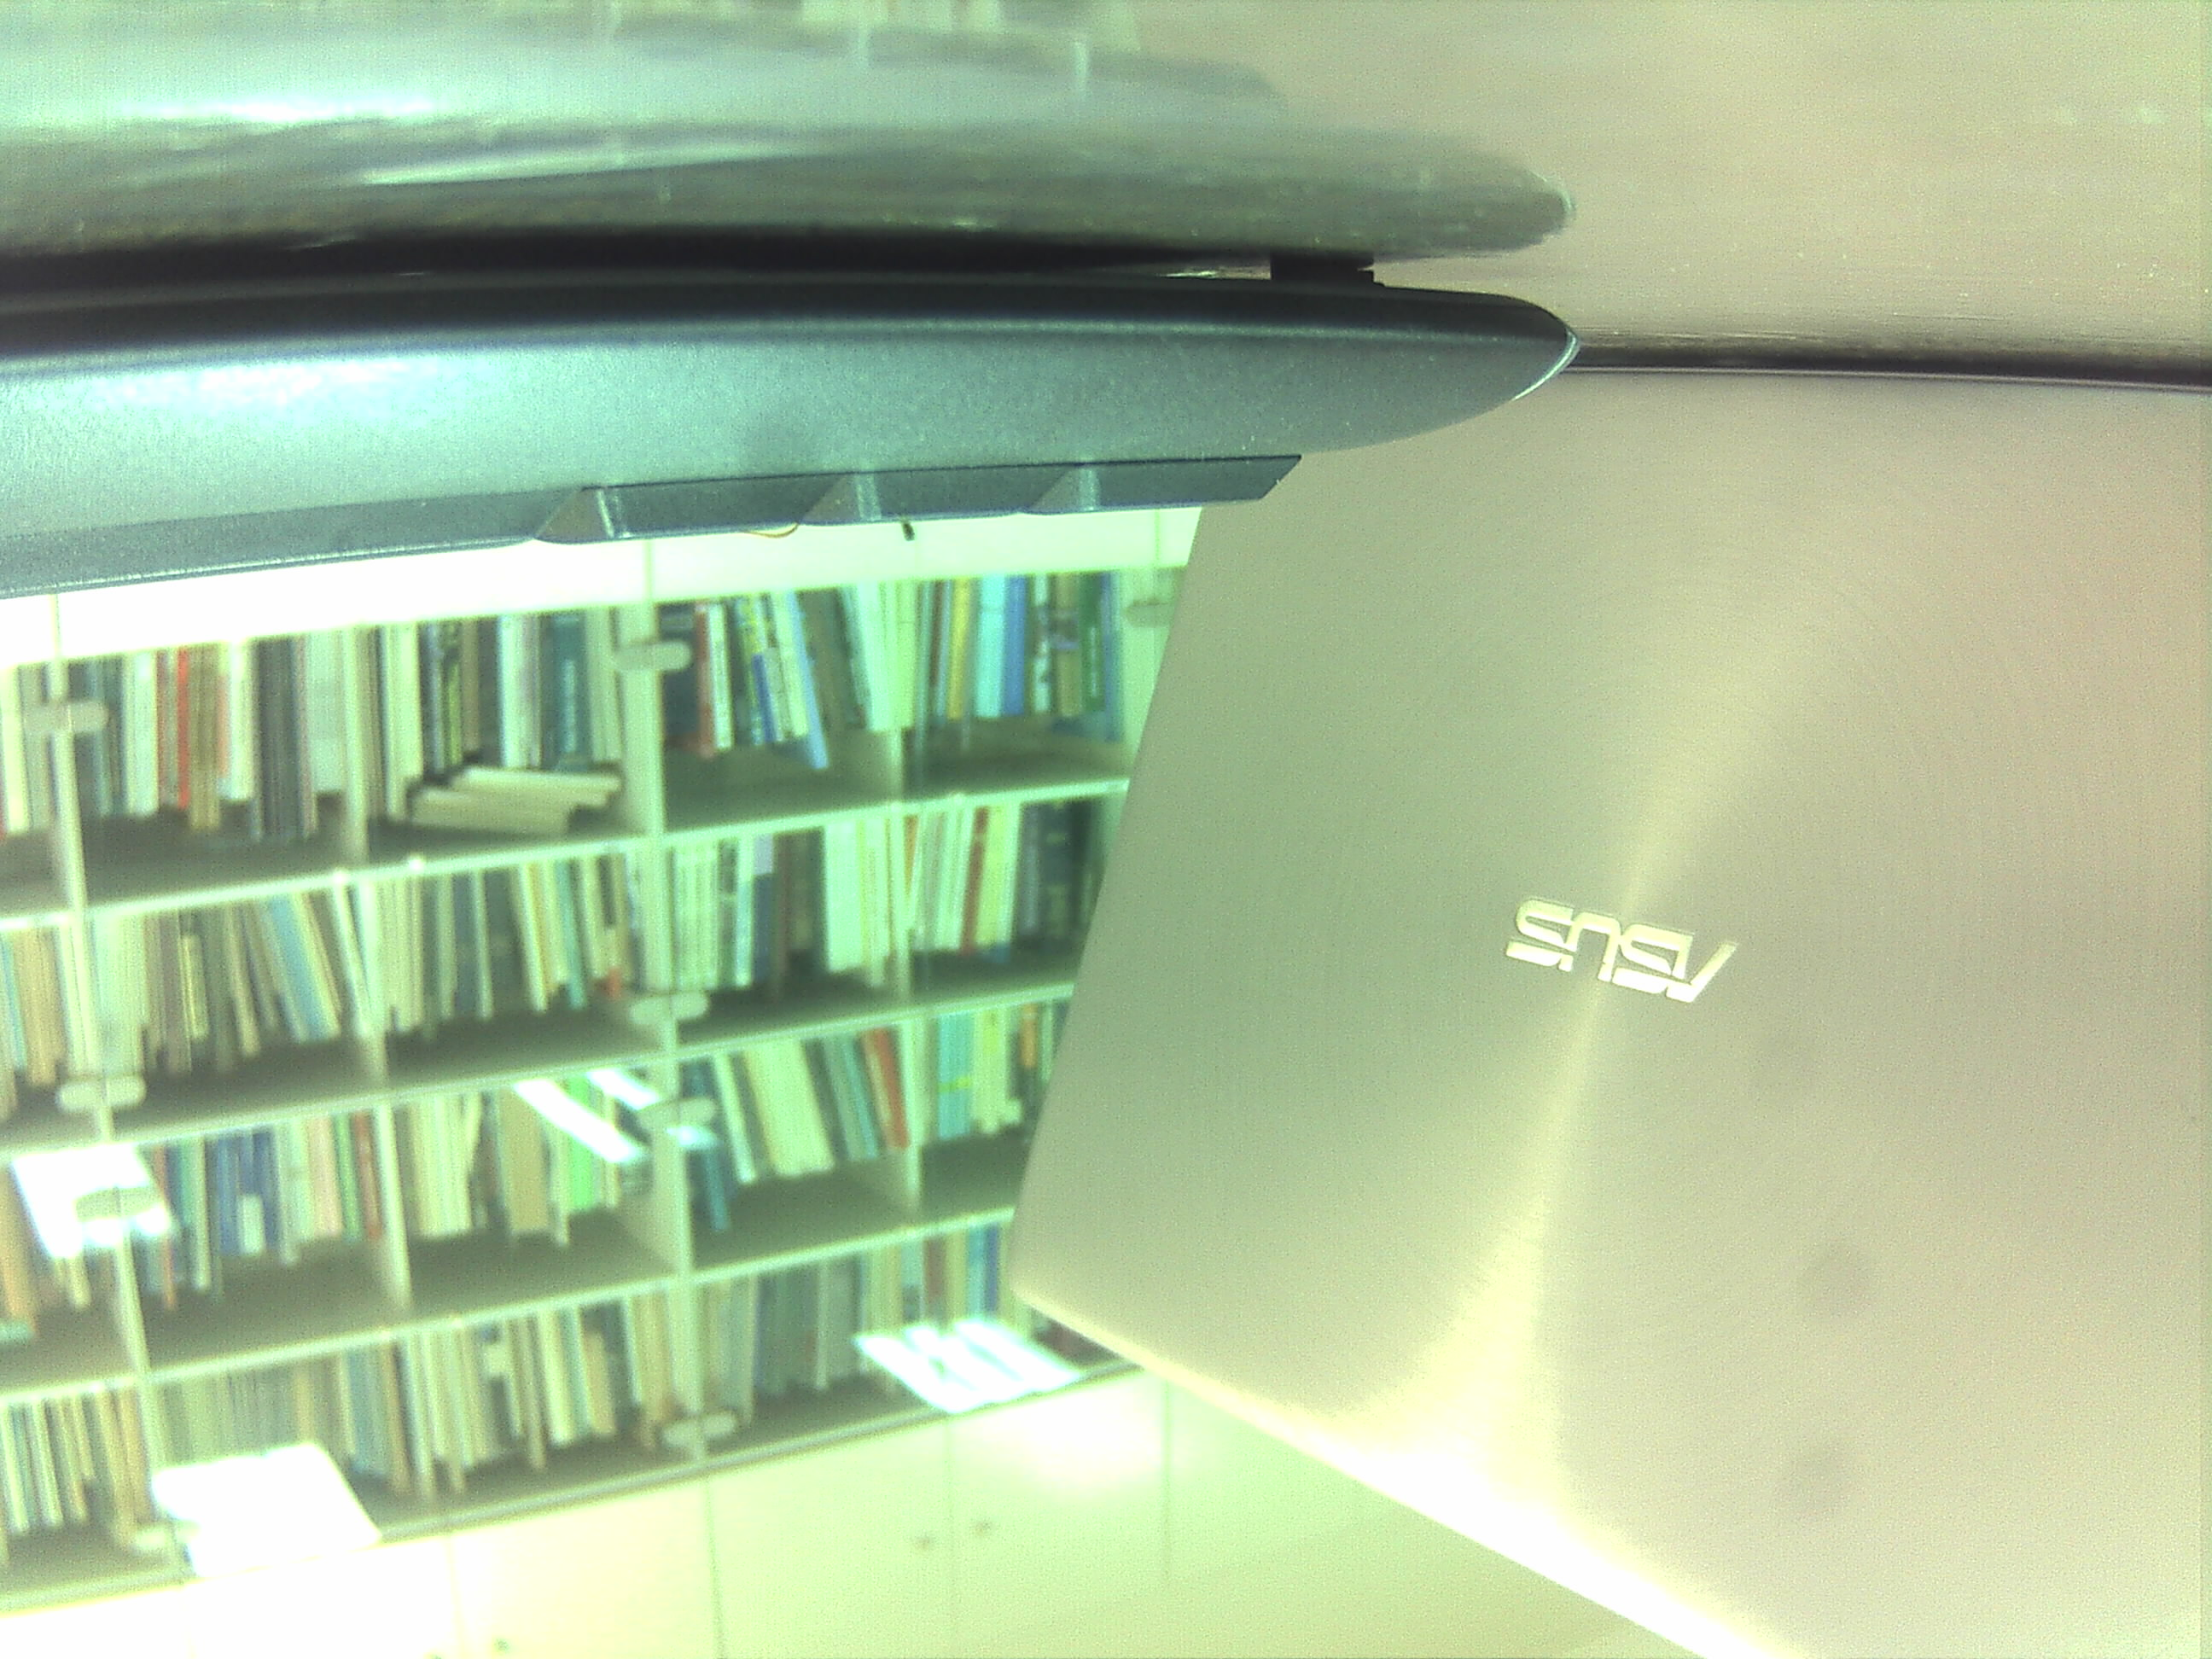
\includegraphics[height=5 cm, angle=180]{light.jpeg}
	\caption{Slika dobivena u relativno svjetlim uvjetima}
	\label{fig:light}
\end{figure}
\begin{figure}[H]
	\centering
	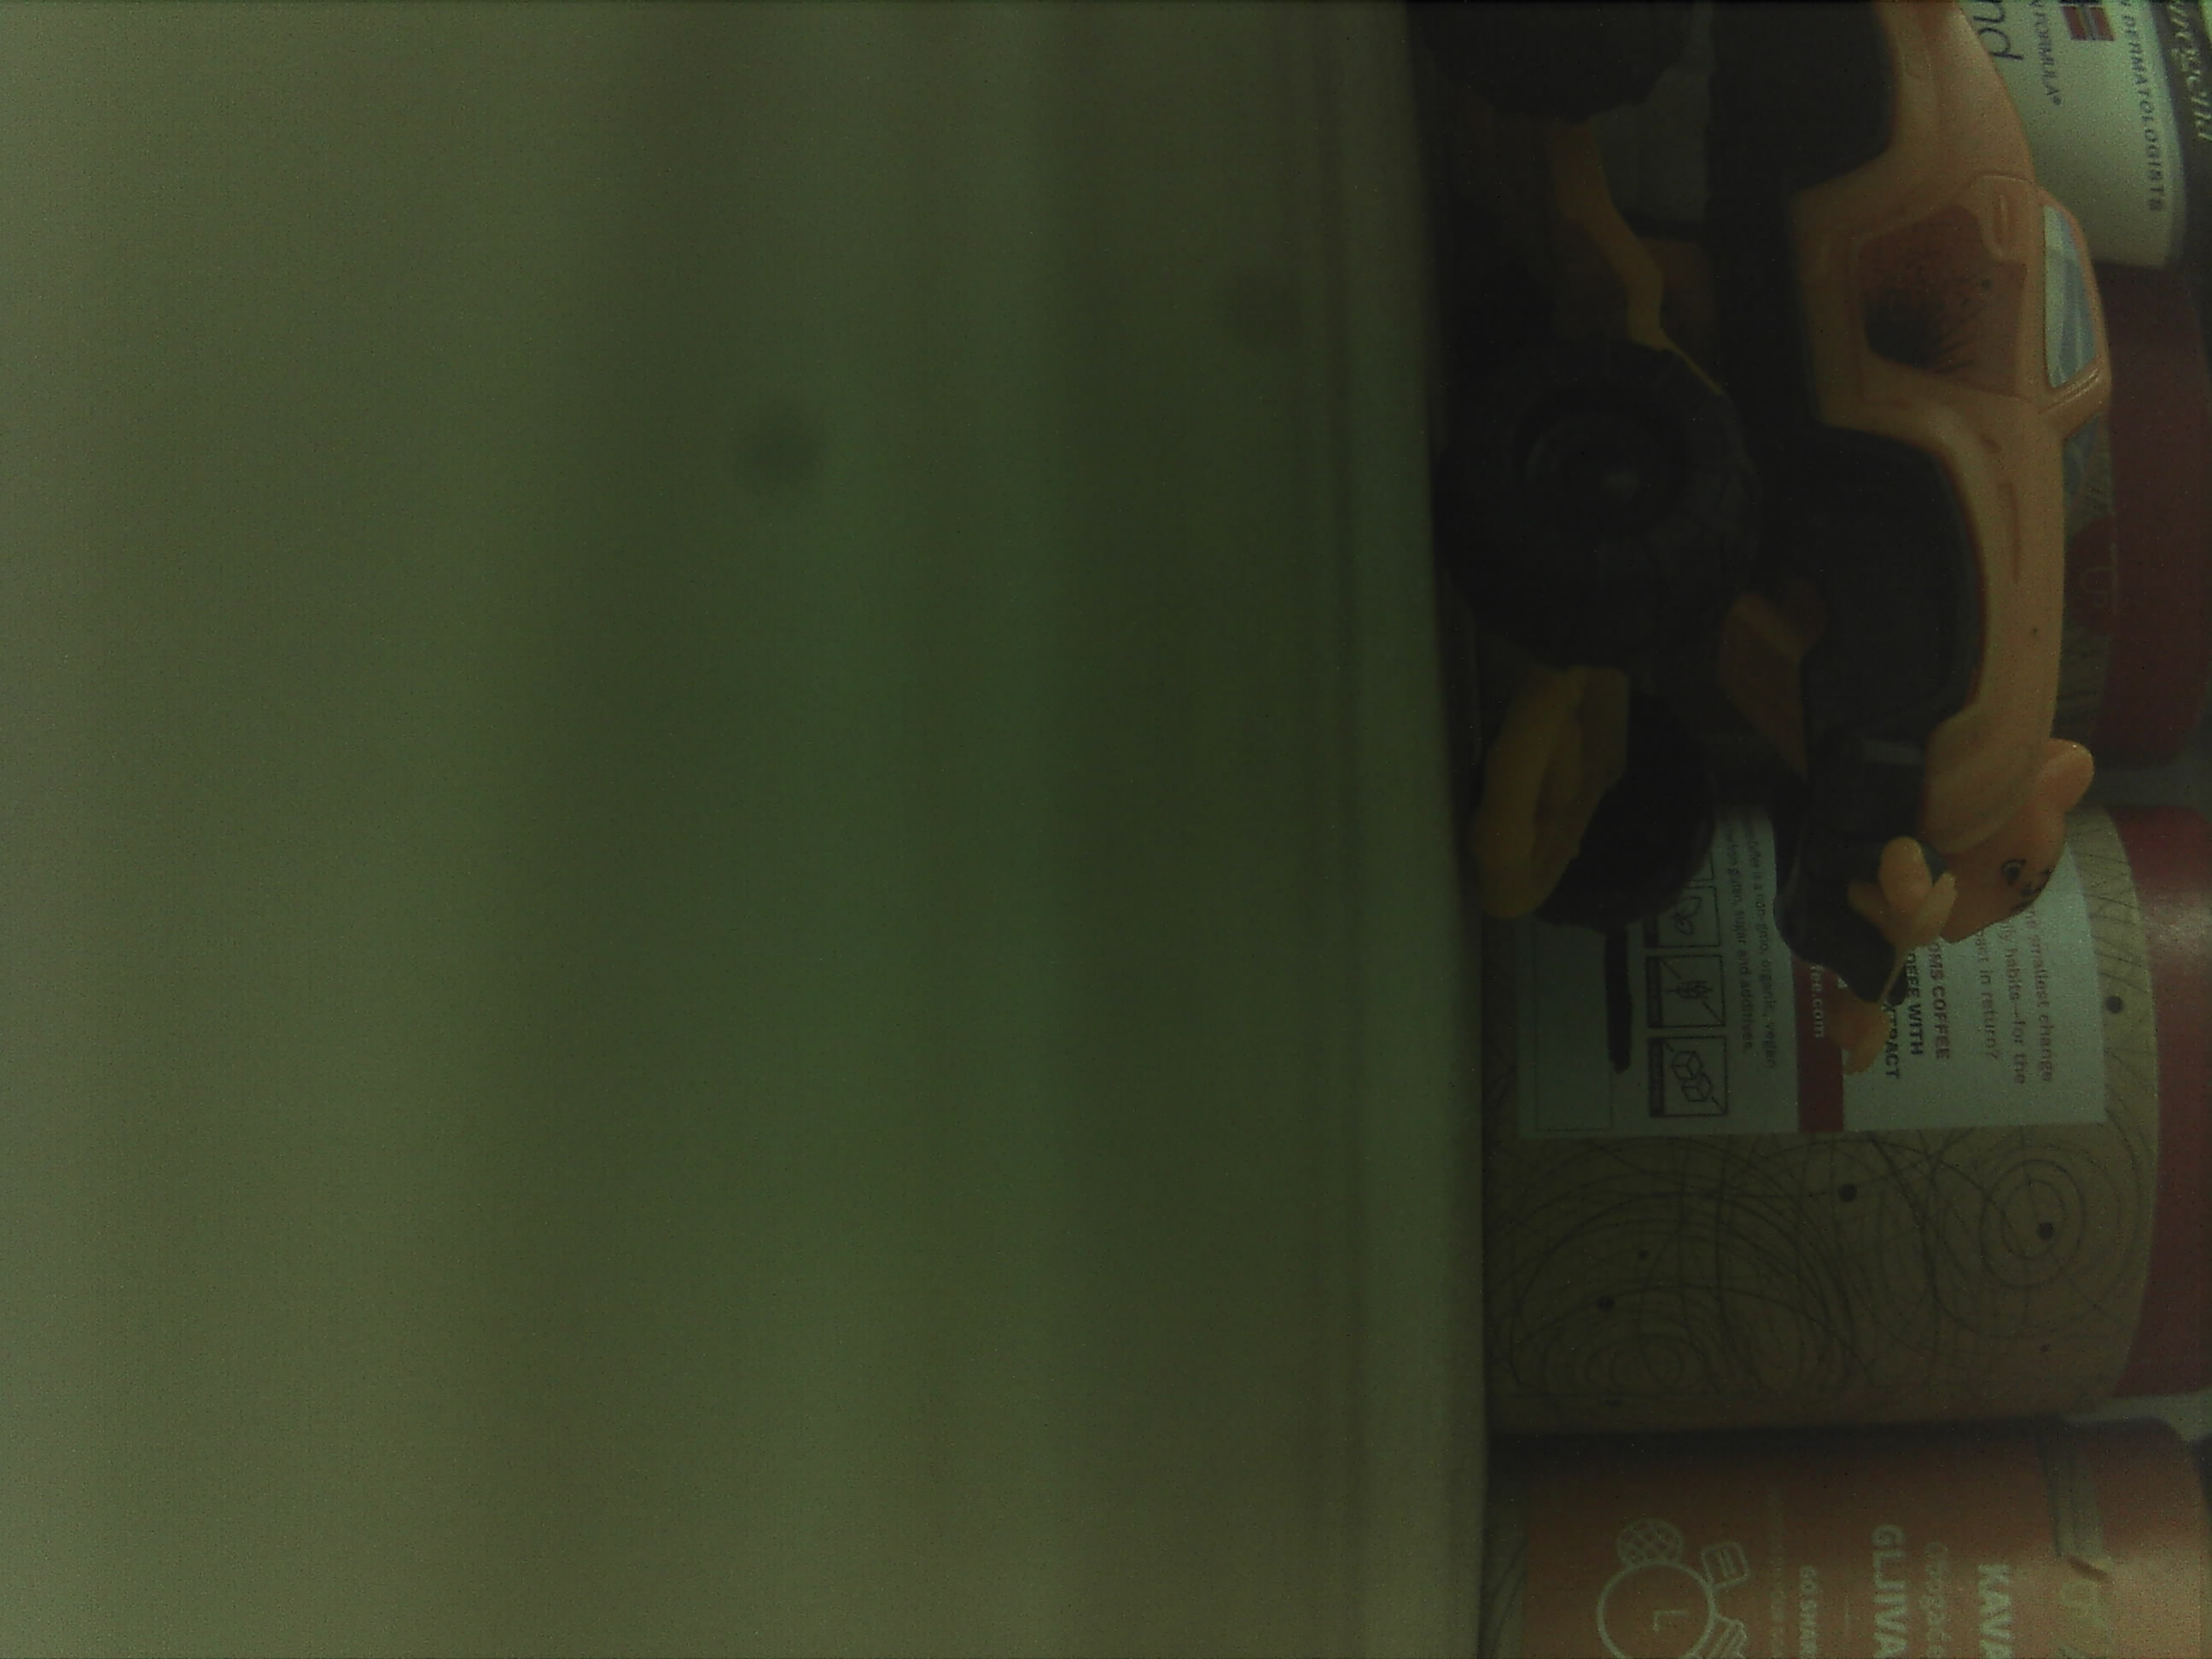
\includegraphics[height=5 cm, angle=90]{dark.jpeg}
	\caption{Slika dobivena u relativno mračnim uvjetima}
	\label{fig:dark}
\end{figure}
\chapter{Zaključak}

\bibliography{literatura}
\bibliographystyle{fer}

\begin{sazetak}
U ovom projektu razvijena je programska podrška za upravljanje kamerom i \textit{flash} memorijom na CubeSat nanosatelitu u sklopu projekta FERSAT. Dan je pregled aktivnosti projekta FERSAT koje su prethodile ovom projektu. Detaljno su opisane SPI i I\textsuperscript{2}C komunikacije pomoću kojih se upravlja kamerom i \textit{flash} memorijom. Dana je usporedba između SPI i I\textsuperscript{2}C periferijskih sklopova STM32F407VGT6 i STM32L471VGT6 mikrokontrolera. Objašnjen je postupak prilagodbe programske podrške s prethodno korištenog (STM32F407VGT6) na trenutačno korišteni (STM32L471VGT6) mikrokontroler. Opisana je integracija razvijene programske podrške u FreeRTOS operacijski sustav za rad u stvarnom vremenu. Objašnjen je način upotrebe CAN periferije ne STM32L471VGT6 mikrokontroleru.

\kljucnerijeci{CubeSat, FERSAT, STM32, kamera, \textit{flash} memorija, programska podrška, SPI, I\textsuperscript{2}C, FreeRTOS, CAN}
\end{sazetak}

% TODO: Navedite naslov na engleskom jeziku.
\engtitle{Software for Camera Control on CubeSat Nanosatellite}
\begin{abstract}
In this project, software support was developed for managing the camera and flash memory on the CubeSat nanosatellite as part of the FERSAT project. An overview of the activities of the FERSAT project that preceded this project was given. The SPI and I\textsuperscript{2}C communications used to control the camera and flash memory are described in detail. A comparison between the SPI and I\textsuperscript{2}C peripheral circuits of STM32F407VGT6 and STM32L471VGT6 microcontrollers is given. The procedure for adapting the firmware from the previously used (STM32F407VGT6) to the currently used (STM32L471VGT6) microcontroller is explained. The integration of the developed software support into the FreeRTOS operating system for real-time operation is described. The method of using the CAN peripherals for the STM32L471VGT6 microcontroller is explained.

\keywords{CubeSat, FERSAT, STM32, camera, flash memory, software support, SPI, I\textsuperscript{2}C, FreeRTOS, CAN}
\end{abstract}

\end{document}
